\documentclass[twoside]{book}

% Packages required by doxygen
\usepackage{calc}
\usepackage{doxygen}
\usepackage{graphicx}
\usepackage[utf8]{inputenc}
\usepackage{makeidx}
\usepackage{multicol}
\usepackage{multirow}
\usepackage{textcomp}
\usepackage[table]{xcolor}

% Font selection
\usepackage[T1]{fontenc}
\usepackage{mathptmx}
\usepackage[scaled=.90]{helvet}
\usepackage{courier}
\usepackage{amssymb}
\usepackage{sectsty}
\renewcommand{\familydefault}{\sfdefault}
\allsectionsfont{%
  \fontseries{bc}\selectfont%
  \color{darkgray}%
}
\renewcommand{\DoxyLabelFont}{%
  \fontseries{bc}\selectfont%
  \color{darkgray}%
}

% Page & text layout
\usepackage{geometry}
\geometry{%
  a4paper,%
  top=2.5cm,%
  bottom=2.5cm,%
  left=2.5cm,%
  right=2.5cm%
}
\tolerance=750
\hfuzz=15pt
\hbadness=750
\setlength{\emergencystretch}{15pt}
\setlength{\parindent}{0cm}
\setlength{\parskip}{0.2cm}
\makeatletter
\renewcommand{\paragraph}{%
  \@startsection{paragraph}{4}{0ex}{-1.0ex}{1.0ex}{%
    \normalfont\normalsize\bfseries\SS@parafont%
  }%
}
\renewcommand{\subparagraph}{%
  \@startsection{subparagraph}{5}{0ex}{-1.0ex}{1.0ex}{%
    \normalfont\normalsize\bfseries\SS@subparafont%
  }%
}
\makeatother

% Headers & footers
\usepackage{fancyhdr}
\pagestyle{fancyplain}
\fancyhead[LE]{\fancyplain{}{\bfseries\thepage}}
\fancyhead[CE]{\fancyplain{}{}}
\fancyhead[RE]{\fancyplain{}{\bfseries\leftmark}}
\fancyhead[LO]{\fancyplain{}{\bfseries\rightmark}}
\fancyhead[CO]{\fancyplain{}{}}
\fancyhead[RO]{\fancyplain{}{\bfseries\thepage}}
\fancyfoot[LE]{\fancyplain{}{}}
\fancyfoot[CE]{\fancyplain{}{}}
\fancyfoot[RE]{\fancyplain{}{\bfseries\scriptsize Generated on Mon Dec 2 2013 10\-:15\-:42 for Bombster by Doxygen }}
\fancyfoot[LO]{\fancyplain{}{\bfseries\scriptsize Generated on Mon Dec 2 2013 10\-:15\-:42 for Bombster by Doxygen }}
\fancyfoot[CO]{\fancyplain{}{}}
\fancyfoot[RO]{\fancyplain{}{}}
\renewcommand{\footrulewidth}{0.4pt}
\renewcommand{\chaptermark}[1]{%
  \markboth{#1}{}%
}
\renewcommand{\sectionmark}[1]{%
  \markright{\thesection\ #1}%
}

% Indices & bibliography
\usepackage{natbib}
\usepackage[titles]{tocloft}
\setcounter{tocdepth}{3}
\setcounter{secnumdepth}{5}
\makeindex

% Hyperlinks (required, but should be loaded last)
\usepackage{ifpdf}
\ifpdf
  \usepackage[pdftex,pagebackref=true]{hyperref}
\else
  \usepackage[ps2pdf,pagebackref=true]{hyperref}
\fi
\hypersetup{%
  colorlinks=true,%
  linkcolor=blue,%
  citecolor=blue,%
  unicode%
}

% Custom commands
\newcommand{\clearemptydoublepage}{%
  \newpage{\pagestyle{empty}\cleardoublepage}%
}


%===== C O N T E N T S =====

\begin{document}

% Titlepage & ToC
\hypersetup{pageanchor=false}
\pagenumbering{roman}
\begin{titlepage}
\vspace*{7cm}
\begin{center}%
{\Large Bombster }\\
\vspace*{1cm}
{\large Generated by Doxygen 1.8.5}\\
\vspace*{0.5cm}
{\small Mon Dec 2 2013 10:15:42}\\
\end{center}
\end{titlepage}
\clearemptydoublepage
\tableofcontents
\clearemptydoublepage
\pagenumbering{arabic}
\hypersetup{pageanchor=true}

%--- Begin generated contents ---
\chapter{Bug List}
\label{bug}
\hypertarget{bug}{}

\begin{DoxyRefList}
\item[\label{bug__bug000001}%
\hypertarget{bug__bug000001}{}%
Member \hyperlink{class_game_screen_af2a5d4c707d0d0f47201eec498b77bd6}{Game\-Screen\-:\-:close\-Event} (Q\-Close\-Event $\ast$)]cannot restart main menu music Closes the current Game and stops music from playing  
\item[\label{bug__bug000002}%
\hypertarget{bug__bug000002}{}%
Member \hyperlink{class_main_window_ab622d7f3b4082b8221185e216991e602}{Main\-Window\-:\-:play\-Again} ()]this is currently not being called Starts up the main menu music. This is to be used after Game music is stopped. 
\end{DoxyRefList}
\chapter{Namespace Index}
\section{Namespace List}
Here is a list of all namespaces with brief descriptions\-:\begin{DoxyCompactList}
\item\contentsline{section}{\hyperlink{namespace_ui}{Ui} }{\pageref{namespace_ui}}{}
\end{DoxyCompactList}

\chapter{Hierarchical Index}
\section{Class Hierarchy}
This inheritance list is sorted roughly, but not completely, alphabetically\-:\begin{DoxyCompactList}
\item Q\-Dialog\begin{DoxyCompactList}
\item \contentsline{section}{Info\-Screen}{\pageref{class_info_screen}}{}
\end{DoxyCompactList}
\item Q\-Graphics\-Object\begin{DoxyCompactList}
\item \contentsline{section}{Block}{\pageref{class_block}}{}
\begin{DoxyCompactList}
\item \contentsline{section}{boxes}{\pageref{classboxes}}{}
\item \contentsline{section}{d\-Wall}{\pageref{classd_wall}}{}
\item \contentsline{section}{Wall}{\pageref{class_wall}}{}
\end{DoxyCompactList}
\item \contentsline{section}{Bomb}{\pageref{class_bomb}}{}
\item \contentsline{section}{Character}{\pageref{class_character}}{}
\item \contentsline{section}{explosion}{\pageref{classexplosion}}{}
\end{DoxyCompactList}
\item Q\-Main\-Window\begin{DoxyCompactList}
\item \contentsline{section}{Game\-Screen}{\pageref{class_game_screen}}{}
\item \contentsline{section}{Main\-Window}{\pageref{class_main_window}}{}
\end{DoxyCompactList}
\item \contentsline{section}{World}{\pageref{class_world}}{}
\end{DoxyCompactList}

\chapter{Class Index}
\section{Class List}
Here are the classes, structs, unions and interfaces with brief descriptions\-:\begin{DoxyCompactList}
\item\contentsline{section}{\hyperlink{class_block}{Block} }{\pageref{class_block}}{}
\item\contentsline{section}{\hyperlink{class_bomb}{Bomb} }{\pageref{class_bomb}}{}
\item\contentsline{section}{\hyperlink{classboxes}{boxes} }{\pageref{classboxes}}{}
\item\contentsline{section}{\hyperlink{class_character}{Character} }{\pageref{class_character}}{}
\item\contentsline{section}{\hyperlink{classd_wall}{d\-Wall} }{\pageref{classd_wall}}{}
\item\contentsline{section}{\hyperlink{classexplosion}{explosion} }{\pageref{classexplosion}}{}
\item\contentsline{section}{\hyperlink{class_game_screen}{Game\-Screen} }{\pageref{class_game_screen}}{}
\item\contentsline{section}{\hyperlink{class_info_screen}{Info\-Screen} }{\pageref{class_info_screen}}{}
\item\contentsline{section}{\hyperlink{class_main_window}{Main\-Window} }{\pageref{class_main_window}}{}
\item\contentsline{section}{\hyperlink{class_wall}{Wall} }{\pageref{class_wall}}{}
\item\contentsline{section}{\hyperlink{class_world}{World} }{\pageref{class_world}}{}
\end{DoxyCompactList}

\chapter{File Index}
\section{File List}
Here is a list of all files with brief descriptions\-:\begin{DoxyCompactList}
\item\contentsline{section}{\hyperlink{block_8cpp}{block.\-cpp} }{\pageref{block_8cpp}}{}
\item\contentsline{section}{\hyperlink{block_8h}{block.\-h} }{\pageref{block_8h}}{}
\item\contentsline{section}{\hyperlink{bomb_8cpp}{bomb.\-cpp} }{\pageref{bomb_8cpp}}{}
\item\contentsline{section}{\hyperlink{bomb_8h}{bomb.\-h} }{\pageref{bomb_8h}}{}
\item\contentsline{section}{\hyperlink{boxes_8cpp}{boxes.\-cpp} }{\pageref{boxes_8cpp}}{}
\item\contentsline{section}{\hyperlink{boxes_8h}{boxes.\-h} }{\pageref{boxes_8h}}{}
\item\contentsline{section}{\hyperlink{character_8cpp}{character.\-cpp} }{\pageref{character_8cpp}}{}
\item\contentsline{section}{\hyperlink{character_8h}{character.\-h} }{\pageref{character_8h}}{}
\item\contentsline{section}{\hyperlink{dwall_8cpp}{dwall.\-cpp} }{\pageref{dwall_8cpp}}{}
\item\contentsline{section}{\hyperlink{dwall_8h}{dwall.\-h} }{\pageref{dwall_8h}}{}
\item\contentsline{section}{\hyperlink{explosion_8cpp}{explosion.\-cpp} }{\pageref{explosion_8cpp}}{}
\item\contentsline{section}{\hyperlink{explosion_8h}{explosion.\-h} }{\pageref{explosion_8h}}{}
\item\contentsline{section}{\hyperlink{gamescreen_8cpp}{gamescreen.\-cpp} }{\pageref{gamescreen_8cpp}}{}
\item\contentsline{section}{\hyperlink{gamescreen_8h}{gamescreen.\-h} }{\pageref{gamescreen_8h}}{}
\item\contentsline{section}{\hyperlink{infoscreen_8cpp}{infoscreen.\-cpp} }{\pageref{infoscreen_8cpp}}{}
\item\contentsline{section}{\hyperlink{infoscreen_8h}{infoscreen.\-h} }{\pageref{infoscreen_8h}}{}
\item\contentsline{section}{\hyperlink{main_8cpp}{main.\-cpp} }{\pageref{main_8cpp}}{}
\item\contentsline{section}{\hyperlink{mainwindow_8cpp}{mainwindow.\-cpp} }{\pageref{mainwindow_8cpp}}{}
\item\contentsline{section}{\hyperlink{mainwindow_8h}{mainwindow.\-h} }{\pageref{mainwindow_8h}}{}
\item\contentsline{section}{\hyperlink{wall_8cpp}{wall.\-cpp} }{\pageref{wall_8cpp}}{}
\item\contentsline{section}{\hyperlink{wall_8h}{wall.\-h} }{\pageref{wall_8h}}{}
\item\contentsline{section}{\hyperlink{world_8cpp}{world.\-cpp} }{\pageref{world_8cpp}}{}
\item\contentsline{section}{\hyperlink{world_8h}{world.\-h} }{\pageref{world_8h}}{}
\end{DoxyCompactList}

\chapter{Namespace Documentation}
\hypertarget{namespace_ui}{\section{Ui Namespace Reference}
\label{namespace_ui}\index{Ui@{Ui}}
}

\chapter{Class Documentation}
\hypertarget{class_block}{\section{Block Class Reference}
\label{class_block}\index{Block@{Block}}
}


{\ttfamily \#include $<$block.\-h$>$}

Inheritance diagram for Block\-:\begin{figure}[H]
\begin{center}
\leavevmode
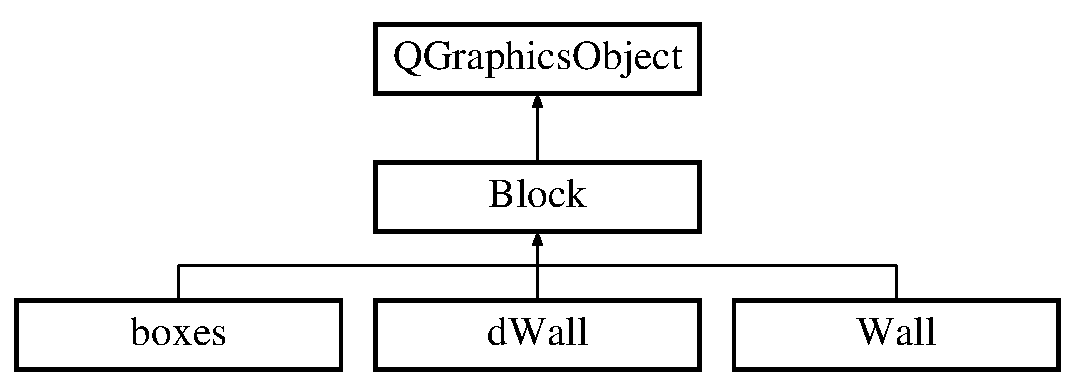
\includegraphics[height=3.000000cm]{class_block}
\end{center}
\end{figure}
\subsection*{Public Member Functions}
\begin{DoxyCompactItemize}
\item 
\hyperlink{class_block_aada344df339d2124eeaa726367ae27fe}{Block} (int x=0, int y=0)
\begin{DoxyCompactList}\small\item\em A Standard \hyperlink{class_block}{Block} This class creates and positions a block into the \hyperlink{class_game_screen}{Game\-Screen}. \end{DoxyCompactList}\item 
virtual \hyperlink{class_block_a19d1bd0e1cef6a865ed2745a2e648405}{$\sim$\-Block} ()
\begin{DoxyCompactList}\small\item\em The \hyperlink{class_block}{Block} destructor Removes a block and prints to console whenever that happens. \end{DoxyCompactList}\item 
virtual void \hyperlink{class_block_aa374e103c2ba9e060c4689f4da21a9ff}{update} (int x, int y)
\begin{DoxyCompactList}\small\item\em Updates a \hyperlink{class_block}{Block} Position. \end{DoxyCompactList}\item 
virtual void \hyperlink{class_block_a8f526f6d76bf11afae85d8b23239cce2}{paint} (Q\-Painter $\ast$painter, const Q\-Style\-Option\-Graphics\-Item $\ast$option, Q\-Widget $\ast$widget)
\item 
virtual Q\-Rect\-F \hyperlink{class_block_aee4444b92a82f5a8080e9019ef1e554d}{bounding\-Rect} () const 
\item 
int \hyperlink{class_block_a527c8f990b4b99dda6f4ca225ee32c14}{get\-X} ()
\begin{DoxyCompactList}\small\item\em Return the X Position of a \hyperlink{class_block}{Block}. \end{DoxyCompactList}\item 
int \hyperlink{class_block_a2501c303a7975db005ddc49d9551a51b}{get\-Y} ()
\begin{DoxyCompactList}\small\item\em Return the Y Position of a \hyperlink{class_block}{Block}. \end{DoxyCompactList}\item 
void \hyperlink{class_block_ab9ac08d83a0e4ff7acb78029df4cc9e2}{set\-X} (int x)
\begin{DoxyCompactList}\small\item\em Set the X Position of a \hyperlink{class_block}{Block}. \end{DoxyCompactList}\item 
void \hyperlink{class_block_a57c1fcfd7d7cda4b9e21d69a25896c17}{set\-Y} (int y)
\begin{DoxyCompactList}\small\item\em Set the Y Position of a \hyperlink{class_block}{Block}. \end{DoxyCompactList}\end{DoxyCompactItemize}
\subsection*{Protected Attributes}
\begin{DoxyCompactItemize}
\item 
qreal \hyperlink{class_block_a97b5b28230920e5f6e3335a023628477}{x\-Pos}
\item 
qreal \hyperlink{class_block_a0857435a94babc54051428becff56867}{y\-Pos}
\end{DoxyCompactItemize}


\subsection{Constructor \& Destructor Documentation}
\hypertarget{class_block_aada344df339d2124eeaa726367ae27fe}{\index{Block@{Block}!Block@{Block}}
\index{Block@{Block}!Block@{Block}}
\subsubsection[{Block}]{\setlength{\rightskip}{0pt plus 5cm}Block\-::\-Block (
\begin{DoxyParamCaption}
\item[{int}]{x = {\ttfamily 0}, }
\item[{int}]{y = {\ttfamily 0}}
\end{DoxyParamCaption}
)}}\label{class_block_aada344df339d2124eeaa726367ae27fe}


A Standard \hyperlink{class_block}{Block} This class creates and positions a block into the \hyperlink{class_game_screen}{Game\-Screen}. 

\hypertarget{class_block_a19d1bd0e1cef6a865ed2745a2e648405}{\index{Block@{Block}!$\sim$\-Block@{$\sim$\-Block}}
\index{$\sim$\-Block@{$\sim$\-Block}!Block@{Block}}
\subsubsection[{$\sim$\-Block}]{\setlength{\rightskip}{0pt plus 5cm}Block\-::$\sim$\-Block (
\begin{DoxyParamCaption}
{}
\end{DoxyParamCaption}
)\hspace{0.3cm}{\ttfamily [virtual]}}}\label{class_block_a19d1bd0e1cef6a865ed2745a2e648405}


The \hyperlink{class_block}{Block} destructor Removes a block and prints to console whenever that happens. 



\subsection{Member Function Documentation}
\hypertarget{class_block_aee4444b92a82f5a8080e9019ef1e554d}{\index{Block@{Block}!bounding\-Rect@{bounding\-Rect}}
\index{bounding\-Rect@{bounding\-Rect}!Block@{Block}}
\subsubsection[{bounding\-Rect}]{\setlength{\rightskip}{0pt plus 5cm}Q\-Rect\-F Block\-::bounding\-Rect (
\begin{DoxyParamCaption}
{}
\end{DoxyParamCaption}
) const\hspace{0.3cm}{\ttfamily [virtual]}}}\label{class_block_aee4444b92a82f5a8080e9019ef1e554d}


Reimplemented in \hyperlink{class_wall_aae7888200bcd5afb12b24110886366a0}{Wall}, \hyperlink{classboxes_a4855400f92db9ebe776a79c79bac1d50}{boxes}, and \hyperlink{classd_wall_a84d4bba890333394f10c5497379d894c}{d\-Wall}.

\hypertarget{class_block_a527c8f990b4b99dda6f4ca225ee32c14}{\index{Block@{Block}!get\-X@{get\-X}}
\index{get\-X@{get\-X}!Block@{Block}}
\subsubsection[{get\-X}]{\setlength{\rightskip}{0pt plus 5cm}int Block\-::get\-X (
\begin{DoxyParamCaption}
{}
\end{DoxyParamCaption}
)}}\label{class_block_a527c8f990b4b99dda6f4ca225ee32c14}


Return the X Position of a \hyperlink{class_block}{Block}. 

\hypertarget{class_block_a2501c303a7975db005ddc49d9551a51b}{\index{Block@{Block}!get\-Y@{get\-Y}}
\index{get\-Y@{get\-Y}!Block@{Block}}
\subsubsection[{get\-Y}]{\setlength{\rightskip}{0pt plus 5cm}int Block\-::get\-Y (
\begin{DoxyParamCaption}
{}
\end{DoxyParamCaption}
)}}\label{class_block_a2501c303a7975db005ddc49d9551a51b}


Return the Y Position of a \hyperlink{class_block}{Block}. 

\hypertarget{class_block_a8f526f6d76bf11afae85d8b23239cce2}{\index{Block@{Block}!paint@{paint}}
\index{paint@{paint}!Block@{Block}}
\subsubsection[{paint}]{\setlength{\rightskip}{0pt plus 5cm}void Block\-::paint (
\begin{DoxyParamCaption}
\item[{Q\-Painter $\ast$}]{painter, }
\item[{const Q\-Style\-Option\-Graphics\-Item $\ast$}]{option, }
\item[{Q\-Widget $\ast$}]{widget}
\end{DoxyParamCaption}
)\hspace{0.3cm}{\ttfamily [virtual]}}}\label{class_block_a8f526f6d76bf11afae85d8b23239cce2}


Reimplemented in \hyperlink{class_wall_aae57ed47f7d5d58b513d2ebd8feb8057}{Wall}, \hyperlink{classboxes_aa07b0460f8be5da676c4369331061fa6}{boxes}, and \hyperlink{classd_wall_aeaec158ea8576bfe6d40d8197ffceaf6}{d\-Wall}.

\hypertarget{class_block_ab9ac08d83a0e4ff7acb78029df4cc9e2}{\index{Block@{Block}!set\-X@{set\-X}}
\index{set\-X@{set\-X}!Block@{Block}}
\subsubsection[{set\-X}]{\setlength{\rightskip}{0pt plus 5cm}void Block\-::set\-X (
\begin{DoxyParamCaption}
\item[{int}]{x}
\end{DoxyParamCaption}
)}}\label{class_block_ab9ac08d83a0e4ff7acb78029df4cc9e2}


Set the X Position of a \hyperlink{class_block}{Block}. 


\begin{DoxyParams}{Parameters}
{\em The} & block's X position \\
\hline
\end{DoxyParams}
\hypertarget{class_block_a57c1fcfd7d7cda4b9e21d69a25896c17}{\index{Block@{Block}!set\-Y@{set\-Y}}
\index{set\-Y@{set\-Y}!Block@{Block}}
\subsubsection[{set\-Y}]{\setlength{\rightskip}{0pt plus 5cm}void Block\-::set\-Y (
\begin{DoxyParamCaption}
\item[{int}]{y}
\end{DoxyParamCaption}
)}}\label{class_block_a57c1fcfd7d7cda4b9e21d69a25896c17}


Set the Y Position of a \hyperlink{class_block}{Block}. 


\begin{DoxyParams}{Parameters}
{\em The} & block's Y position \\
\hline
\end{DoxyParams}
\hypertarget{class_block_aa374e103c2ba9e060c4689f4da21a9ff}{\index{Block@{Block}!update@{update}}
\index{update@{update}!Block@{Block}}
\subsubsection[{update}]{\setlength{\rightskip}{0pt plus 5cm}void Block\-::update (
\begin{DoxyParamCaption}
\item[{int}]{x, }
\item[{int}]{y}
\end{DoxyParamCaption}
)\hspace{0.3cm}{\ttfamily [virtual]}}}\label{class_block_aa374e103c2ba9e060c4689f4da21a9ff}


Updates a \hyperlink{class_block}{Block} Position. 


\begin{DoxyParams}{Parameters}
{\em x} & position \\
\hline
{\em y} & position This updates the position of the block \\
\hline
\end{DoxyParams}


\subsection{Member Data Documentation}
\hypertarget{class_block_a97b5b28230920e5f6e3335a023628477}{\index{Block@{Block}!x\-Pos@{x\-Pos}}
\index{x\-Pos@{x\-Pos}!Block@{Block}}
\subsubsection[{x\-Pos}]{\setlength{\rightskip}{0pt plus 5cm}qreal Block\-::x\-Pos\hspace{0.3cm}{\ttfamily [protected]}}}\label{class_block_a97b5b28230920e5f6e3335a023628477}
\hypertarget{class_block_a0857435a94babc54051428becff56867}{\index{Block@{Block}!y\-Pos@{y\-Pos}}
\index{y\-Pos@{y\-Pos}!Block@{Block}}
\subsubsection[{y\-Pos}]{\setlength{\rightskip}{0pt plus 5cm}qreal Block\-::y\-Pos\hspace{0.3cm}{\ttfamily [protected]}}}\label{class_block_a0857435a94babc54051428becff56867}


The documentation for this class was generated from the following files\-:\begin{DoxyCompactItemize}
\item 
\hyperlink{block_8h}{block.\-h}\item 
\hyperlink{block_8cpp}{block.\-cpp}\end{DoxyCompactItemize}

\hypertarget{class_bomb}{\section{Bomb Class Reference}
\label{class_bomb}\index{Bomb@{Bomb}}
}


Inheritance diagram for Bomb\-:


Collaboration diagram for Bomb\-:
\subsection*{Public Slots}
\begin{DoxyCompactItemize}
\item 
\hypertarget{class_bomb_a5752ce7daece5c3bf2e2178bcfcb820d}{void {\bfseries explode} ()}\label{class_bomb_a5752ce7daece5c3bf2e2178bcfcb820d}

\item 
\hypertarget{class_bomb_ae9410dc9b499dad8e4f0f200d9b0ead7}{void {\bfseries explode2} ()}\label{class_bomb_ae9410dc9b499dad8e4f0f200d9b0ead7}

\end{DoxyCompactItemize}
\subsection*{Public Member Functions}
\begin{DoxyCompactItemize}
\item 
\hypertarget{class_bomb_ada9d05fb30c035691190e80d1d0a1c7f}{{\bfseries Bomb} (int x=0, int y=0, int explosion\-Size=0)}\label{class_bomb_ada9d05fb30c035691190e80d1d0a1c7f}

\item 
\hypertarget{class_bomb_ad047941e8f1413a061f98f460dcea22a}{Q\-Rect\-F {\bfseries bounding\-Rect} () const }\label{class_bomb_ad047941e8f1413a061f98f460dcea22a}

\item 
\hypertarget{class_bomb_ab8e930cc66f5d3f41e8a02f3d0d8185e}{void {\bfseries paint} (Q\-Painter $\ast$painter, const Q\-Style\-Option\-Graphics\-Item $\ast$option, Q\-Widget $\ast$widget)}\label{class_bomb_ab8e930cc66f5d3f41e8a02f3d0d8185e}

\end{DoxyCompactItemize}
\subsection*{Protected Attributes}
\begin{DoxyCompactItemize}
\item 
\hypertarget{class_bomb_ac2068167b771ed338aa17c99524b8131}{qreal {\bfseries x\-Pos}}\label{class_bomb_ac2068167b771ed338aa17c99524b8131}

\item 
\hypertarget{class_bomb_a0d1028a49b33b08f5c96a943fab0beff}{qreal {\bfseries y\-Pos}}\label{class_bomb_a0d1028a49b33b08f5c96a943fab0beff}

\item 
\hypertarget{class_bomb_a7576bf99d4bcfbc7dda365511ca2fcd7}{int {\bfseries explosion\-Size}}\label{class_bomb_a7576bf99d4bcfbc7dda365511ca2fcd7}

\item 
\hypertarget{class_bomb_a03d27f3d615aba4b77f83427912a7de6}{std\-::vector$<$ \hyperlink{classexplosion}{explosion} $\ast$ $>$ {\bfseries explosion\-Vector}}\label{class_bomb_a03d27f3d615aba4b77f83427912a7de6}

\end{DoxyCompactItemize}


The documentation for this class was generated from the following files\-:\begin{DoxyCompactItemize}
\item 
bomb.\-h\item 
bomb.\-cpp\end{DoxyCompactItemize}

\hypertarget{classboxes}{\section{boxes Class Reference}
\label{classboxes}\index{boxes@{boxes}}
}


{\ttfamily \#include $<$boxes.\-h$>$}

Inheritance diagram for boxes\-:\begin{figure}[H]
\begin{center}
\leavevmode
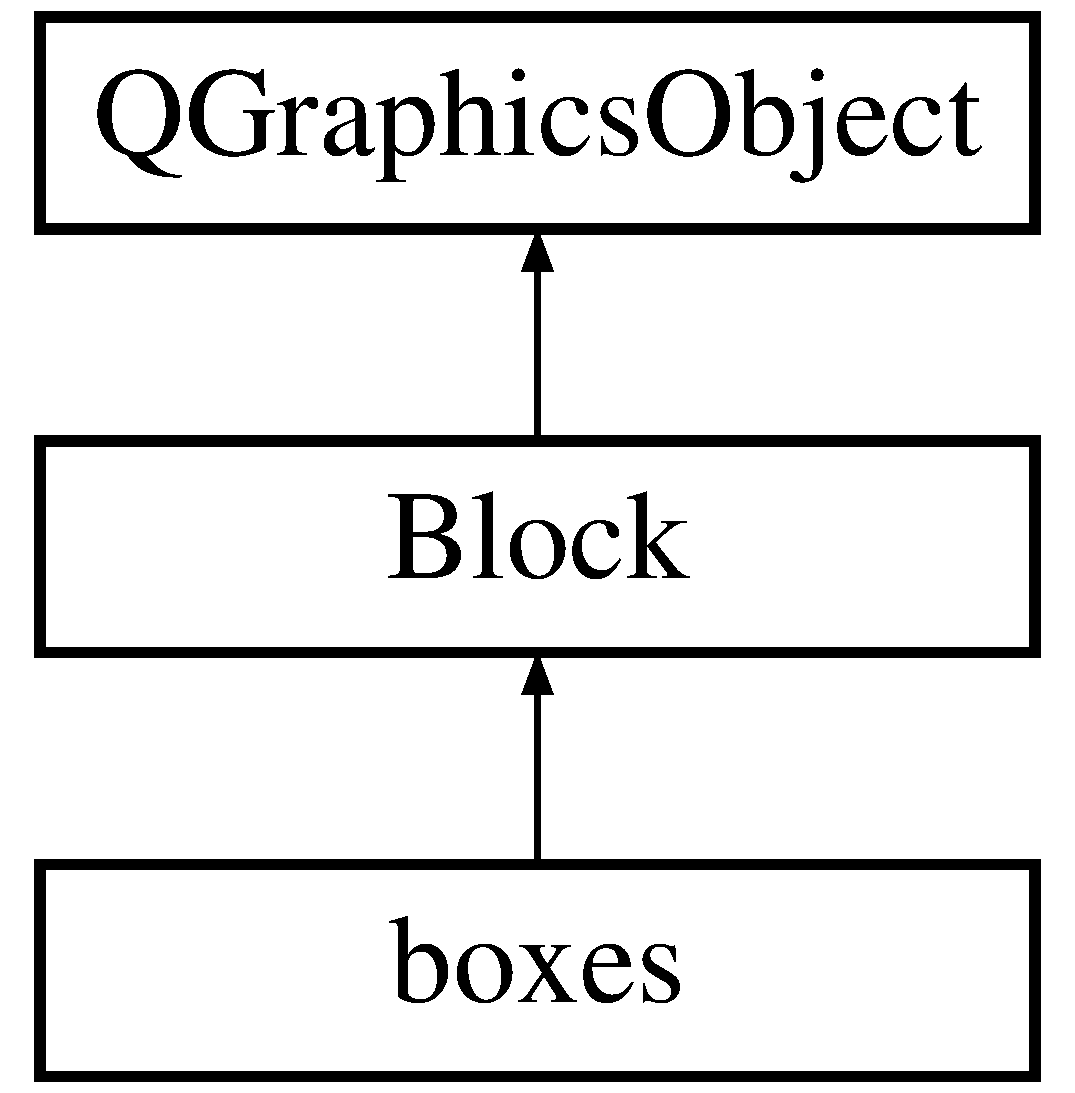
\includegraphics[height=3.000000cm]{classboxes}
\end{center}
\end{figure}
\subsection*{Public Member Functions}
\begin{DoxyCompactItemize}
\item 
\hyperlink{classboxes_a093427b27f4b84a803544cb738dc12e6}{boxes} (int x=0, int y=0)
\begin{DoxyCompactList}\small\item\em this class creates a box \end{DoxyCompactList}\item 
\hyperlink{classboxes_a7d70921b4fe775ad313ac80d6da55222}{$\sim$boxes} ()
\begin{DoxyCompactList}\small\item\em The boxes destructor Removes a box and prints to console whenever that happens. \end{DoxyCompactList}\item 
void \hyperlink{classboxes_aa07b0460f8be5da676c4369331061fa6}{paint} (Q\-Painter $\ast$painter, const Q\-Style\-Option\-Graphics\-Item $\ast$option, Q\-Widget $\ast$widget)
\item 
Q\-Rect\-F \hyperlink{classboxes_a4855400f92db9ebe776a79c79bac1d50}{bounding\-Rect} () const 
\end{DoxyCompactItemize}
\subsection*{Protected Attributes}
\begin{DoxyCompactItemize}
\item 
int \hyperlink{classboxes_a2600eb866b188f33fb6415fc358f449a}{type}
\end{DoxyCompactItemize}


\subsection{Constructor \& Destructor Documentation}
\hypertarget{classboxes_a093427b27f4b84a803544cb738dc12e6}{\index{boxes@{boxes}!boxes@{boxes}}
\index{boxes@{boxes}!boxes@{boxes}}
\subsubsection[{boxes}]{\setlength{\rightskip}{0pt plus 5cm}boxes\-::boxes (
\begin{DoxyParamCaption}
\item[{int}]{x = {\ttfamily 0}, }
\item[{int}]{y = {\ttfamily 0}}
\end{DoxyParamCaption}
)}}\label{classboxes_a093427b27f4b84a803544cb738dc12e6}


this class creates a box 


\begin{DoxyParams}{Parameters}
{\em the} & x coordinate in the world \\
\hline
{\em the} & y coordinate in the world creates a box with they x and y coordinate given and notes it in the console \\
\hline
\end{DoxyParams}
\hypertarget{classboxes_a7d70921b4fe775ad313ac80d6da55222}{\index{boxes@{boxes}!$\sim$boxes@{$\sim$boxes}}
\index{$\sim$boxes@{$\sim$boxes}!boxes@{boxes}}
\subsubsection[{$\sim$boxes}]{\setlength{\rightskip}{0pt plus 5cm}boxes\-::$\sim$boxes (
\begin{DoxyParamCaption}
{}
\end{DoxyParamCaption}
)}}\label{classboxes_a7d70921b4fe775ad313ac80d6da55222}


The boxes destructor Removes a box and prints to console whenever that happens. 



\subsection{Member Function Documentation}
\hypertarget{classboxes_a4855400f92db9ebe776a79c79bac1d50}{\index{boxes@{boxes}!bounding\-Rect@{bounding\-Rect}}
\index{bounding\-Rect@{bounding\-Rect}!boxes@{boxes}}
\subsubsection[{bounding\-Rect}]{\setlength{\rightskip}{0pt plus 5cm}Q\-Rect\-F boxes\-::bounding\-Rect (
\begin{DoxyParamCaption}
{}
\end{DoxyParamCaption}
) const\hspace{0.3cm}{\ttfamily [virtual]}}}\label{classboxes_a4855400f92db9ebe776a79c79bac1d50}


Reimplemented from \hyperlink{class_block_aee4444b92a82f5a8080e9019ef1e554d}{Block}.

\hypertarget{classboxes_aa07b0460f8be5da676c4369331061fa6}{\index{boxes@{boxes}!paint@{paint}}
\index{paint@{paint}!boxes@{boxes}}
\subsubsection[{paint}]{\setlength{\rightskip}{0pt plus 5cm}void boxes\-::paint (
\begin{DoxyParamCaption}
\item[{Q\-Painter $\ast$}]{painter, }
\item[{const Q\-Style\-Option\-Graphics\-Item $\ast$}]{option, }
\item[{Q\-Widget $\ast$}]{widget}
\end{DoxyParamCaption}
)\hspace{0.3cm}{\ttfamily [virtual]}}}\label{classboxes_aa07b0460f8be5da676c4369331061fa6}


Reimplemented from \hyperlink{class_block_a8f526f6d76bf11afae85d8b23239cce2}{Block}.



\subsection{Member Data Documentation}
\hypertarget{classboxes_a2600eb866b188f33fb6415fc358f449a}{\index{boxes@{boxes}!type@{type}}
\index{type@{type}!boxes@{boxes}}
\subsubsection[{type}]{\setlength{\rightskip}{0pt plus 5cm}int boxes\-::type\hspace{0.3cm}{\ttfamily [protected]}}}\label{classboxes_a2600eb866b188f33fb6415fc358f449a}


The documentation for this class was generated from the following files\-:\begin{DoxyCompactItemize}
\item 
\hyperlink{boxes_8h}{boxes.\-h}\item 
\hyperlink{boxes_8cpp}{boxes.\-cpp}\end{DoxyCompactItemize}

\hypertarget{class_character}{\section{Character Class Reference}
\label{class_character}\index{Character@{Character}}
}


The \hyperlink{class_character}{Character} class of Bombster used to create a movable player in the world.  




{\ttfamily \#include $<$character.\-h$>$}

Inheritance diagram for Character\-:\begin{figure}[H]
\begin{center}
\leavevmode
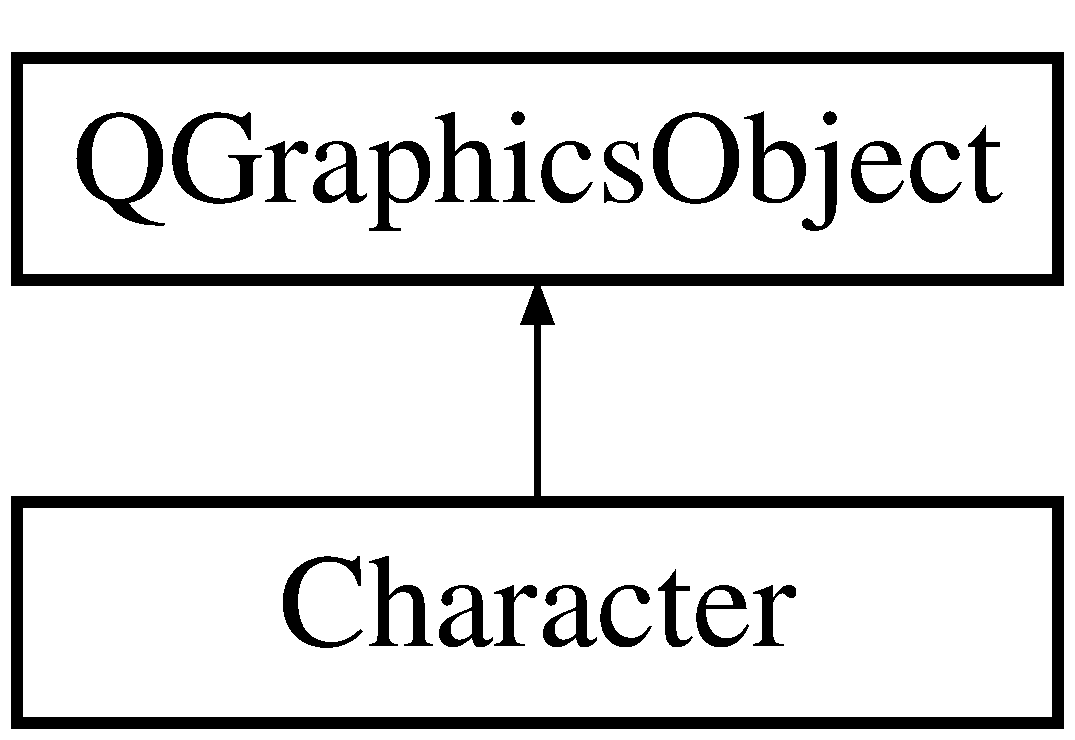
\includegraphics[height=2.000000cm]{class_character}
\end{center}
\end{figure}
\subsection*{Public Member Functions}
\begin{DoxyCompactItemize}
\item 
\hyperlink{class_character_ade1bb6dc548f73fb814702776457a1f3}{Character} (int x=0, int y=0, int num\-Bombs=3, int player=-\/1)
\begin{DoxyCompactList}\small\item\em The \hyperlink{class_character}{Character} constructer. \end{DoxyCompactList}\item 
\hyperlink{class_character_a9e9be564d05ded80962b2045aa70b3fc}{$\sim$\-Character} ()
\begin{DoxyCompactList}\small\item\em The \hyperlink{class_character}{Character} destructor Removes a \hyperlink{class_character}{Character} and prints to console whenever that happens. \end{DoxyCompactList}\item 
void \hyperlink{class_character_a5e63747ea61305391cd0ada0898e485c}{move\-Up} ()
\begin{DoxyCompactList}\small\item\em moves a character Up a 1/2 block. \end{DoxyCompactList}\item 
void \hyperlink{class_character_afa7763e81bca6a0b9b0c044f39c429f0}{move\-Down} ()
\begin{DoxyCompactList}\small\item\em Moves a \hyperlink{class_character}{Character} down a 1/2 block. \end{DoxyCompactList}\item 
void \hyperlink{class_character_a88dfc867ab226d3f115b891fc3b34d67}{move\-Left} ()
\begin{DoxyCompactList}\small\item\em Moves a \hyperlink{class_character}{Character} Left a 1/2 block. \end{DoxyCompactList}\item 
void \hyperlink{class_character_a0a8bf66e3d70c196a0fa8ce183f4aeb4}{move\-Right} ()
\begin{DoxyCompactList}\small\item\em Moves a \hyperlink{class_character}{Character} Right a 1/2 block. \end{DoxyCompactList}\item 
void \hyperlink{class_character_a38747fb2a1e186e6cc871f0836eb83e8}{drop\-Bomb} ()
\begin{DoxyCompactList}\small\item\em Allows the \hyperlink{class_character}{Character} to drop a \hyperlink{class_bomb}{Bomb}. Places a bomb in the Game where the \hyperlink{class_character}{Character} currently is placed and starts the ountdown to the explosion. \end{DoxyCompactList}\item 
void \hyperlink{class_character_acb99685904de8dce448ad8a51efed7cb}{picked\-Up} (int item)
\item 
int \hyperlink{class_character_aacb2a15ce71f1165daceb29cf481a4cb}{get\-Player\-I\-D} ()
\begin{DoxyCompactList}\small\item\em gets a Player I\-D \end{DoxyCompactList}\item 
void \hyperlink{class_character_a099916c7331625461d7cd976ec4b0498}{paint} (Q\-Painter $\ast$painter, const Q\-Style\-Option\-Graphics\-Item $\ast$option, Q\-Widget $\ast$widget)
\item 
Q\-Rect\-F \hyperlink{class_character_af3bf8c7fe7ddbad47b54193374d25ee2}{bounding\-Rect} () const 
\item 
int \hyperlink{class_character_aba58d60bcfe61c1807e1a9e9439b56f0}{type} () const 
\end{DoxyCompactItemize}


\subsection{Detailed Description}
The \hyperlink{class_character}{Character} class of Bombster used to create a movable player in the world. 

Inherits Q\-Graphics\-Object from Qt 

\subsection{Constructor \& Destructor Documentation}
\hypertarget{class_character_ade1bb6dc548f73fb814702776457a1f3}{\index{Character@{Character}!Character@{Character}}
\index{Character@{Character}!Character@{Character}}
\subsubsection[{Character}]{\setlength{\rightskip}{0pt plus 5cm}Character\-::\-Character (
\begin{DoxyParamCaption}
\item[{int}]{x = {\ttfamily 0}, }
\item[{int}]{y = {\ttfamily 0}, }
\item[{int}]{num\-Bombs = {\ttfamily 3}, }
\item[{int}]{player = {\ttfamily -\/1}}
\end{DoxyParamCaption}
)}}\label{class_character_ade1bb6dc548f73fb814702776457a1f3}


The \hyperlink{class_character}{Character} constructer. 


\begin{DoxyParams}{Parameters}
{\em The} & x coordinate of where the player currently is. \\
\hline
{\em The} & y coordinate of where the player currently is. \\
\hline
{\em The} & initial number of bombs the character may have. \\
\hline
{\em The} & player\-I\-D. this constructor creates a character given a position in the world, the amount of bombs the character can have, and the player\-I\-D \\
\hline
\end{DoxyParams}
\hypertarget{class_character_a9e9be564d05ded80962b2045aa70b3fc}{\index{Character@{Character}!$\sim$\-Character@{$\sim$\-Character}}
\index{$\sim$\-Character@{$\sim$\-Character}!Character@{Character}}
\subsubsection[{$\sim$\-Character}]{\setlength{\rightskip}{0pt plus 5cm}Character\-::$\sim$\-Character (
\begin{DoxyParamCaption}
{}
\end{DoxyParamCaption}
)}}\label{class_character_a9e9be564d05ded80962b2045aa70b3fc}


The \hyperlink{class_character}{Character} destructor Removes a \hyperlink{class_character}{Character} and prints to console whenever that happens. 



\subsection{Member Function Documentation}
\hypertarget{class_character_af3bf8c7fe7ddbad47b54193374d25ee2}{\index{Character@{Character}!bounding\-Rect@{bounding\-Rect}}
\index{bounding\-Rect@{bounding\-Rect}!Character@{Character}}
\subsubsection[{bounding\-Rect}]{\setlength{\rightskip}{0pt plus 5cm}Q\-Rect\-F Character\-::bounding\-Rect (
\begin{DoxyParamCaption}
{}
\end{DoxyParamCaption}
) const}}\label{class_character_af3bf8c7fe7ddbad47b54193374d25ee2}
\hypertarget{class_character_a38747fb2a1e186e6cc871f0836eb83e8}{\index{Character@{Character}!drop\-Bomb@{drop\-Bomb}}
\index{drop\-Bomb@{drop\-Bomb}!Character@{Character}}
\subsubsection[{drop\-Bomb}]{\setlength{\rightskip}{0pt plus 5cm}void Character\-::drop\-Bomb (
\begin{DoxyParamCaption}
{}
\end{DoxyParamCaption}
)}}\label{class_character_a38747fb2a1e186e6cc871f0836eb83e8}


Allows the \hyperlink{class_character}{Character} to drop a \hyperlink{class_bomb}{Bomb}. Places a bomb in the Game where the \hyperlink{class_character}{Character} currently is placed and starts the ountdown to the explosion. 

\hypertarget{class_character_aacb2a15ce71f1165daceb29cf481a4cb}{\index{Character@{Character}!get\-Player\-I\-D@{get\-Player\-I\-D}}
\index{get\-Player\-I\-D@{get\-Player\-I\-D}!Character@{Character}}
\subsubsection[{get\-Player\-I\-D}]{\setlength{\rightskip}{0pt plus 5cm}int Character\-::get\-Player\-I\-D (
\begin{DoxyParamCaption}
{}
\end{DoxyParamCaption}
)}}\label{class_character_aacb2a15ce71f1165daceb29cf481a4cb}


gets a Player I\-D 

\begin{DoxyReturn}{Returns}
Returns the \hyperlink{class_character}{Character}'s player\-I\-D 
\end{DoxyReturn}
\hypertarget{class_character_afa7763e81bca6a0b9b0c044f39c429f0}{\index{Character@{Character}!move\-Down@{move\-Down}}
\index{move\-Down@{move\-Down}!Character@{Character}}
\subsubsection[{move\-Down}]{\setlength{\rightskip}{0pt plus 5cm}void Character\-::move\-Down (
\begin{DoxyParamCaption}
{}
\end{DoxyParamCaption}
)}}\label{class_character_afa7763e81bca6a0b9b0c044f39c429f0}


Moves a \hyperlink{class_character}{Character} down a 1/2 block. 

\hypertarget{class_character_a88dfc867ab226d3f115b891fc3b34d67}{\index{Character@{Character}!move\-Left@{move\-Left}}
\index{move\-Left@{move\-Left}!Character@{Character}}
\subsubsection[{move\-Left}]{\setlength{\rightskip}{0pt plus 5cm}void Character\-::move\-Left (
\begin{DoxyParamCaption}
{}
\end{DoxyParamCaption}
)}}\label{class_character_a88dfc867ab226d3f115b891fc3b34d67}


Moves a \hyperlink{class_character}{Character} Left a 1/2 block. 

\hypertarget{class_character_a0a8bf66e3d70c196a0fa8ce183f4aeb4}{\index{Character@{Character}!move\-Right@{move\-Right}}
\index{move\-Right@{move\-Right}!Character@{Character}}
\subsubsection[{move\-Right}]{\setlength{\rightskip}{0pt plus 5cm}void Character\-::move\-Right (
\begin{DoxyParamCaption}
{}
\end{DoxyParamCaption}
)}}\label{class_character_a0a8bf66e3d70c196a0fa8ce183f4aeb4}


Moves a \hyperlink{class_character}{Character} Right a 1/2 block. 

\hypertarget{class_character_a5e63747ea61305391cd0ada0898e485c}{\index{Character@{Character}!move\-Up@{move\-Up}}
\index{move\-Up@{move\-Up}!Character@{Character}}
\subsubsection[{move\-Up}]{\setlength{\rightskip}{0pt plus 5cm}void Character\-::move\-Up (
\begin{DoxyParamCaption}
{}
\end{DoxyParamCaption}
)}}\label{class_character_a5e63747ea61305391cd0ada0898e485c}


moves a character Up a 1/2 block. 

\hypertarget{class_character_a099916c7331625461d7cd976ec4b0498}{\index{Character@{Character}!paint@{paint}}
\index{paint@{paint}!Character@{Character}}
\subsubsection[{paint}]{\setlength{\rightskip}{0pt plus 5cm}void Character\-::paint (
\begin{DoxyParamCaption}
\item[{Q\-Painter $\ast$}]{painter, }
\item[{const Q\-Style\-Option\-Graphics\-Item $\ast$}]{option, }
\item[{Q\-Widget $\ast$}]{widget}
\end{DoxyParamCaption}
)}}\label{class_character_a099916c7331625461d7cd976ec4b0498}
\hypertarget{class_character_acb99685904de8dce448ad8a51efed7cb}{\index{Character@{Character}!picked\-Up@{picked\-Up}}
\index{picked\-Up@{picked\-Up}!Character@{Character}}
\subsubsection[{picked\-Up}]{\setlength{\rightskip}{0pt plus 5cm}void Character\-::picked\-Up (
\begin{DoxyParamCaption}
\item[{int}]{item}
\end{DoxyParamCaption}
)}}\label{class_character_acb99685904de8dce448ad8a51efed7cb}
\hypertarget{class_character_aba58d60bcfe61c1807e1a9e9439b56f0}{\index{Character@{Character}!type@{type}}
\index{type@{type}!Character@{Character}}
\subsubsection[{type}]{\setlength{\rightskip}{0pt plus 5cm}int Character\-::type (
\begin{DoxyParamCaption}
{}
\end{DoxyParamCaption}
) const}}\label{class_character_aba58d60bcfe61c1807e1a9e9439b56f0}


The documentation for this class was generated from the following files\-:\begin{DoxyCompactItemize}
\item 
\hyperlink{character_8h}{character.\-h}\item 
\hyperlink{character_8cpp}{character.\-cpp}\end{DoxyCompactItemize}

\hypertarget{classd_wall}{\section{d\-Wall Class Reference}
\label{classd_wall}\index{d\-Wall@{d\-Wall}}
}


{\ttfamily \#include $<$dwall.\-h$>$}

Inheritance diagram for d\-Wall\-:\begin{figure}[H]
\begin{center}
\leavevmode
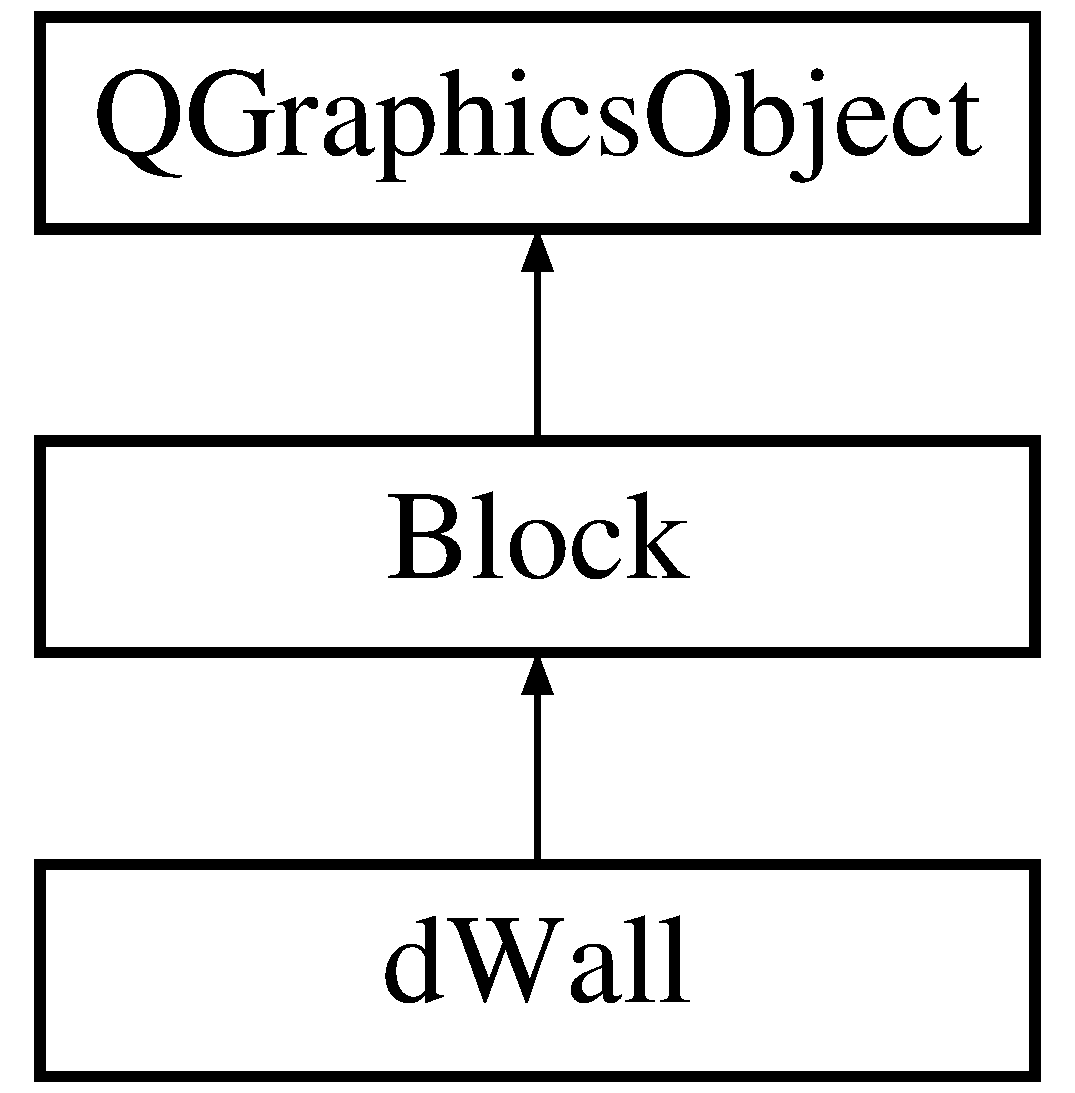
\includegraphics[height=3.000000cm]{classd_wall}
\end{center}
\end{figure}
\subsection*{Public Member Functions}
\begin{DoxyCompactItemize}
\item 
\hyperlink{classd_wall_a09862932157c8e5f8a59b22b3222d816}{d\-Wall} (int x=0, int y=0)
\begin{DoxyCompactList}\small\item\em Destructable wall constructor. \end{DoxyCompactList}\item 
\hyperlink{classd_wall_ae3e072cee7b80cf20387c3d634cb994a}{$\sim$d\-Wall} ()
\begin{DoxyCompactList}\small\item\em The Destructable \hyperlink{class_wall}{Wall} destructor Removes a Destructable \hyperlink{class_wall}{Wall} from the game and prints to console whenever that happens. \end{DoxyCompactList}\item 
void \hyperlink{classd_wall_aeaec158ea8576bfe6d40d8197ffceaf6}{paint} (Q\-Painter $\ast$painter, const Q\-Style\-Option\-Graphics\-Item $\ast$option, Q\-Widget $\ast$widget)
\item 
Q\-Rect\-F \hyperlink{classd_wall_a84d4bba890333394f10c5497379d894c}{bounding\-Rect} () const 
\end{DoxyCompactItemize}
\subsection*{Additional Inherited Members}


\subsection{Constructor \& Destructor Documentation}
\hypertarget{classd_wall_a09862932157c8e5f8a59b22b3222d816}{\index{d\-Wall@{d\-Wall}!d\-Wall@{d\-Wall}}
\index{d\-Wall@{d\-Wall}!dWall@{d\-Wall}}
\subsubsection[{d\-Wall}]{\setlength{\rightskip}{0pt plus 5cm}d\-Wall\-::d\-Wall (
\begin{DoxyParamCaption}
\item[{int}]{x = {\ttfamily 0}, }
\item[{int}]{y = {\ttfamily 0}}
\end{DoxyParamCaption}
)}}\label{classd_wall_a09862932157c8e5f8a59b22b3222d816}


Destructable wall constructor. 


\begin{DoxyParams}{Parameters}
{\em the} & x Position in the \hyperlink{class_world}{World} \\
\hline
{\em the} & y Position in the \hyperlink{class_world}{World} Given Coordinates, this constuctor creates a destructable \hyperlink{class_wall}{Wall} and prints to console whenever that happens \\
\hline
\end{DoxyParams}
\hypertarget{classd_wall_ae3e072cee7b80cf20387c3d634cb994a}{\index{d\-Wall@{d\-Wall}!$\sim$d\-Wall@{$\sim$d\-Wall}}
\index{$\sim$d\-Wall@{$\sim$d\-Wall}!dWall@{d\-Wall}}
\subsubsection[{$\sim$d\-Wall}]{\setlength{\rightskip}{0pt plus 5cm}d\-Wall\-::$\sim$d\-Wall (
\begin{DoxyParamCaption}
{}
\end{DoxyParamCaption}
)}}\label{classd_wall_ae3e072cee7b80cf20387c3d634cb994a}


The Destructable \hyperlink{class_wall}{Wall} destructor Removes a Destructable \hyperlink{class_wall}{Wall} from the game and prints to console whenever that happens. 



\subsection{Member Function Documentation}
\hypertarget{classd_wall_a84d4bba890333394f10c5497379d894c}{\index{d\-Wall@{d\-Wall}!bounding\-Rect@{bounding\-Rect}}
\index{bounding\-Rect@{bounding\-Rect}!dWall@{d\-Wall}}
\subsubsection[{bounding\-Rect}]{\setlength{\rightskip}{0pt plus 5cm}Q\-Rect\-F d\-Wall\-::bounding\-Rect (
\begin{DoxyParamCaption}
{}
\end{DoxyParamCaption}
) const\hspace{0.3cm}{\ttfamily [virtual]}}}\label{classd_wall_a84d4bba890333394f10c5497379d894c}


Reimplemented from \hyperlink{class_block_aee4444b92a82f5a8080e9019ef1e554d}{Block}.

\hypertarget{classd_wall_aeaec158ea8576bfe6d40d8197ffceaf6}{\index{d\-Wall@{d\-Wall}!paint@{paint}}
\index{paint@{paint}!dWall@{d\-Wall}}
\subsubsection[{paint}]{\setlength{\rightskip}{0pt plus 5cm}void d\-Wall\-::paint (
\begin{DoxyParamCaption}
\item[{Q\-Painter $\ast$}]{painter, }
\item[{const Q\-Style\-Option\-Graphics\-Item $\ast$}]{option, }
\item[{Q\-Widget $\ast$}]{widget}
\end{DoxyParamCaption}
)\hspace{0.3cm}{\ttfamily [virtual]}}}\label{classd_wall_aeaec158ea8576bfe6d40d8197ffceaf6}


Reimplemented from \hyperlink{class_block_a8f526f6d76bf11afae85d8b23239cce2}{Block}.



The documentation for this class was generated from the following files\-:\begin{DoxyCompactItemize}
\item 
\hyperlink{dwall_8h}{dwall.\-h}\item 
\hyperlink{dwall_8cpp}{dwall.\-cpp}\end{DoxyCompactItemize}

\hypertarget{classexplosion}{\section{explosion Class Reference}
\label{classexplosion}\index{explosion@{explosion}}
}


{\ttfamily \#include $<$explosion.\-h$>$}

Inheritance diagram for explosion\-:\begin{figure}[H]
\begin{center}
\leavevmode
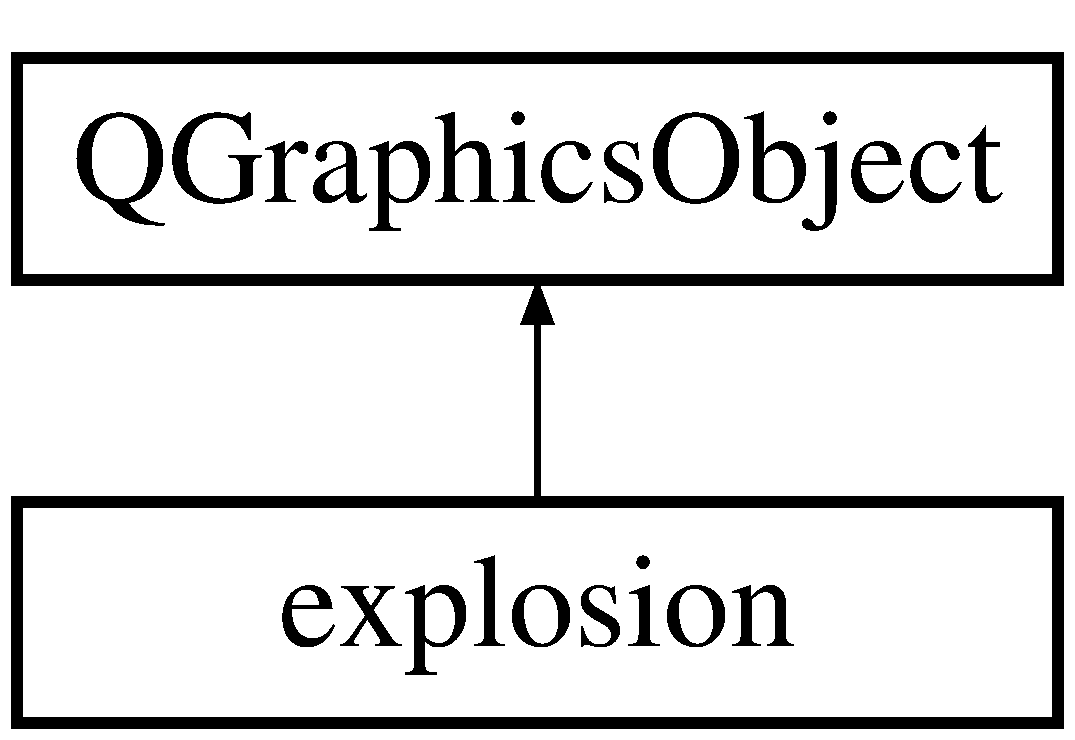
\includegraphics[height=2.000000cm]{classexplosion}
\end{center}
\end{figure}
\subsection*{Public Member Functions}
\begin{DoxyCompactItemize}
\item 
\hyperlink{classexplosion_ac3aabcbf16f356fcd3bdc8588cf36cf1}{explosion} (int x=0, int y=0)
\item 
\hyperlink{classexplosion_a3fc08d8c702d74ee3164825c975f8230}{$\sim$explosion} ()
\begin{DoxyCompactList}\small\item\em The Explosion destructor Removes an explosion and prints to console whenever that happens. \end{DoxyCompactList}\item 
Q\-Rect\-F \hyperlink{classexplosion_adc8680178e9e7d4e388d8850a2c03125}{bounding\-Rect} () const 
\item 
void \hyperlink{classexplosion_a401d7dbebfc4a92bcc408172df67c782}{paint} (Q\-Painter $\ast$painter, const Q\-Style\-Option\-Graphics\-Item $\ast$option, Q\-Widget $\ast$widget)
\end{DoxyCompactItemize}


\subsection{Constructor \& Destructor Documentation}
\hypertarget{classexplosion_ac3aabcbf16f356fcd3bdc8588cf36cf1}{\index{explosion@{explosion}!explosion@{explosion}}
\index{explosion@{explosion}!explosion@{explosion}}
\subsubsection[{explosion}]{\setlength{\rightskip}{0pt plus 5cm}explosion\-::explosion (
\begin{DoxyParamCaption}
\item[{int}]{x = {\ttfamily 0}, }
\item[{int}]{y = {\ttfamily 0}}
\end{DoxyParamCaption}
)}}\label{classexplosion_ac3aabcbf16f356fcd3bdc8588cf36cf1}
\hypertarget{classexplosion_a3fc08d8c702d74ee3164825c975f8230}{\index{explosion@{explosion}!$\sim$explosion@{$\sim$explosion}}
\index{$\sim$explosion@{$\sim$explosion}!explosion@{explosion}}
\subsubsection[{$\sim$explosion}]{\setlength{\rightskip}{0pt plus 5cm}explosion\-::$\sim$explosion (
\begin{DoxyParamCaption}
{}
\end{DoxyParamCaption}
)}}\label{classexplosion_a3fc08d8c702d74ee3164825c975f8230}


The Explosion destructor Removes an explosion and prints to console whenever that happens. 



\subsection{Member Function Documentation}
\hypertarget{classexplosion_adc8680178e9e7d4e388d8850a2c03125}{\index{explosion@{explosion}!bounding\-Rect@{bounding\-Rect}}
\index{bounding\-Rect@{bounding\-Rect}!explosion@{explosion}}
\subsubsection[{bounding\-Rect}]{\setlength{\rightskip}{0pt plus 5cm}Q\-Rect\-F explosion\-::bounding\-Rect (
\begin{DoxyParamCaption}
{}
\end{DoxyParamCaption}
) const}}\label{classexplosion_adc8680178e9e7d4e388d8850a2c03125}
\hypertarget{classexplosion_a401d7dbebfc4a92bcc408172df67c782}{\index{explosion@{explosion}!paint@{paint}}
\index{paint@{paint}!explosion@{explosion}}
\subsubsection[{paint}]{\setlength{\rightskip}{0pt plus 5cm}void explosion\-::paint (
\begin{DoxyParamCaption}
\item[{Q\-Painter $\ast$}]{painter, }
\item[{const Q\-Style\-Option\-Graphics\-Item $\ast$}]{option, }
\item[{Q\-Widget $\ast$}]{widget}
\end{DoxyParamCaption}
)}}\label{classexplosion_a401d7dbebfc4a92bcc408172df67c782}


The documentation for this class was generated from the following files\-:\begin{DoxyCompactItemize}
\item 
\hyperlink{explosion_8h}{explosion.\-h}\item 
\hyperlink{explosion_8cpp}{explosion.\-cpp}\end{DoxyCompactItemize}

\hypertarget{class_game_screen}{\section{Game\-Screen Class Reference}
\label{class_game_screen}\index{Game\-Screen@{Game\-Screen}}
}


Inheritance diagram for Game\-Screen\-:


Collaboration diagram for Game\-Screen\-:
\subsection*{Public Member Functions}
\begin{DoxyCompactItemize}
\item 
\hypertarget{class_game_screen_a61ac084a564d45be53337cc364214a60}{\hyperlink{class_game_screen_a61ac084a564d45be53337cc364214a60}{Game\-Screen} (Q\-Widget $\ast$parent=0)}\label{class_game_screen_a61ac084a564d45be53337cc364214a60}

\begin{DoxyCompactList}\small\item\em A Gamescreen Object This class creates the game U\-I and sets up background music. \end{DoxyCompactList}\item 
\hypertarget{class_game_screen_a0d25dfce42d72954aab40dbccbf1a0b1}{\hyperlink{class_game_screen_a0d25dfce42d72954aab40dbccbf1a0b1}{$\sim$\-Game\-Screen} ()}\label{class_game_screen_a0d25dfce42d72954aab40dbccbf1a0b1}

\begin{DoxyCompactList}\small\item\em A Gamescreen Destructor The abstract parent of all chess pieces. \end{DoxyCompactList}\item 
\hypertarget{class_game_screen_ab954f12aa342e80cb55dd4e2b8d3afeb}{void {\bfseries paint\-Event} (Q\-Paint\-Event $\ast$event)}\label{class_game_screen_ab954f12aa342e80cb55dd4e2b8d3afeb}

\item 
void \hyperlink{class_game_screen_af2a5d4c707d0d0f47201eec498b77bd6}{close\-Event} (Q\-Close\-Event $\ast$)
\begin{DoxyCompactList}\small\item\em Closing window event. \end{DoxyCompactList}\end{DoxyCompactItemize}
\subsection*{Public Attributes}
\begin{DoxyCompactItemize}
\item 
\hypertarget{class_game_screen_af1416b1a2647d06d0777b863be9c090e}{Q\-Graphics\-Scene $\ast$ {\bfseries scene}}\label{class_game_screen_af1416b1a2647d06d0777b863be9c090e}

\end{DoxyCompactItemize}


\subsection{Member Function Documentation}
\hypertarget{class_game_screen_af2a5d4c707d0d0f47201eec498b77bd6}{\index{Game\-Screen@{Game\-Screen}!close\-Event@{close\-Event}}
\index{close\-Event@{close\-Event}!GameScreen@{Game\-Screen}}
\subsubsection[{close\-Event}]{\setlength{\rightskip}{0pt plus 5cm}void Game\-Screen\-::close\-Event (
\begin{DoxyParamCaption}
\item[{Q\-Close\-Event $\ast$}]{bar}
\end{DoxyParamCaption}
)}}\label{class_game_screen_af2a5d4c707d0d0f47201eec498b77bd6}


Closing window event. 

\begin{DoxyRefDesc}{Bug}
\item[\hyperlink{bug__bug000001}{Bug}]cannot restart main menu music Closes the current Game and stops music from playing \end{DoxyRefDesc}


The documentation for this class was generated from the following files\-:\begin{DoxyCompactItemize}
\item 
gamescreen.\-h\item 
gamescreen.\-cpp\end{DoxyCompactItemize}

\hypertarget{class_info_screen}{\section{Info\-Screen Class Reference}
\label{class_info_screen}\index{Info\-Screen@{Info\-Screen}}
}


The \hyperlink{class_info_screen}{Info\-Screen} class of Bombster used to give information and credits about the game.  




{\ttfamily \#include $<$infoscreen.\-h$>$}

Inheritance diagram for Info\-Screen\-:\begin{figure}[H]
\begin{center}
\leavevmode
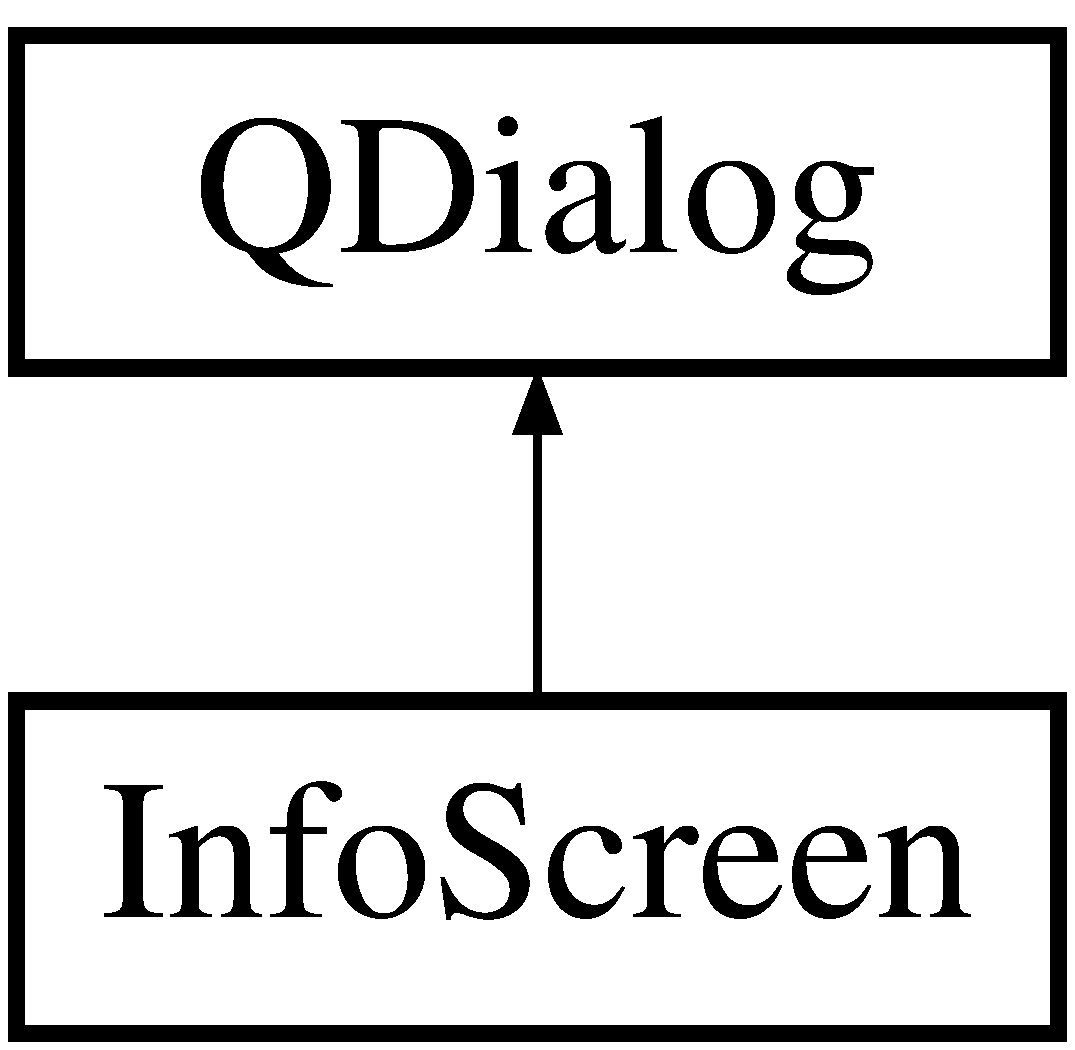
\includegraphics[height=2.000000cm]{class_info_screen}
\end{center}
\end{figure}
\subsection*{Public Member Functions}
\begin{DoxyCompactItemize}
\item 
\hyperlink{class_info_screen_a334bc1b328e13d04889b2f166806de9e}{Info\-Screen} (Q\-Widget $\ast$parent=0)
\begin{DoxyCompactList}\small\item\em The \hyperlink{class_info_screen}{Info\-Screen} constructor Creates the \hyperlink{class_info_screen}{Info\-Screen} U\-I. \end{DoxyCompactList}\item 
\hyperlink{class_info_screen_adc57e13bff37154e1db3346d1ef5c77a}{$\sim$\-Info\-Screen} ()
\begin{DoxyCompactList}\small\item\em The \hyperlink{class_info_screen}{Info\-Screen} destructor Deletes the \hyperlink{class_info_screen}{Info\-Screen} U\-I. \end{DoxyCompactList}\end{DoxyCompactItemize}


\subsection{Detailed Description}
The \hyperlink{class_info_screen}{Info\-Screen} class of Bombster used to give information and credits about the game. 

Inherits Q\-Dialog from Qt 

\subsection{Constructor \& Destructor Documentation}
\hypertarget{class_info_screen_a334bc1b328e13d04889b2f166806de9e}{\index{Info\-Screen@{Info\-Screen}!Info\-Screen@{Info\-Screen}}
\index{Info\-Screen@{Info\-Screen}!InfoScreen@{Info\-Screen}}
\subsubsection[{Info\-Screen}]{\setlength{\rightskip}{0pt plus 5cm}Info\-Screen\-::\-Info\-Screen (
\begin{DoxyParamCaption}
\item[{Q\-Widget $\ast$}]{parent = {\ttfamily 0}}
\end{DoxyParamCaption}
)\hspace{0.3cm}{\ttfamily [explicit]}}}\label{class_info_screen_a334bc1b328e13d04889b2f166806de9e}


The \hyperlink{class_info_screen}{Info\-Screen} constructor Creates the \hyperlink{class_info_screen}{Info\-Screen} U\-I. 

\hypertarget{class_info_screen_adc57e13bff37154e1db3346d1ef5c77a}{\index{Info\-Screen@{Info\-Screen}!$\sim$\-Info\-Screen@{$\sim$\-Info\-Screen}}
\index{$\sim$\-Info\-Screen@{$\sim$\-Info\-Screen}!InfoScreen@{Info\-Screen}}
\subsubsection[{$\sim$\-Info\-Screen}]{\setlength{\rightskip}{0pt plus 5cm}Info\-Screen\-::$\sim$\-Info\-Screen (
\begin{DoxyParamCaption}
{}
\end{DoxyParamCaption}
)}}\label{class_info_screen_adc57e13bff37154e1db3346d1ef5c77a}


The \hyperlink{class_info_screen}{Info\-Screen} destructor Deletes the \hyperlink{class_info_screen}{Info\-Screen} U\-I. 



The documentation for this class was generated from the following files\-:\begin{DoxyCompactItemize}
\item 
\hyperlink{infoscreen_8h}{infoscreen.\-h}\item 
\hyperlink{infoscreen_8cpp}{infoscreen.\-cpp}\end{DoxyCompactItemize}

\hypertarget{class_main_window}{\section{Main\-Window Class Reference}
\label{class_main_window}\index{Main\-Window@{Main\-Window}}
}


{\ttfamily \#include $<$mainwindow.\-h$>$}

Inheritance diagram for Main\-Window\-:\begin{figure}[H]
\begin{center}
\leavevmode
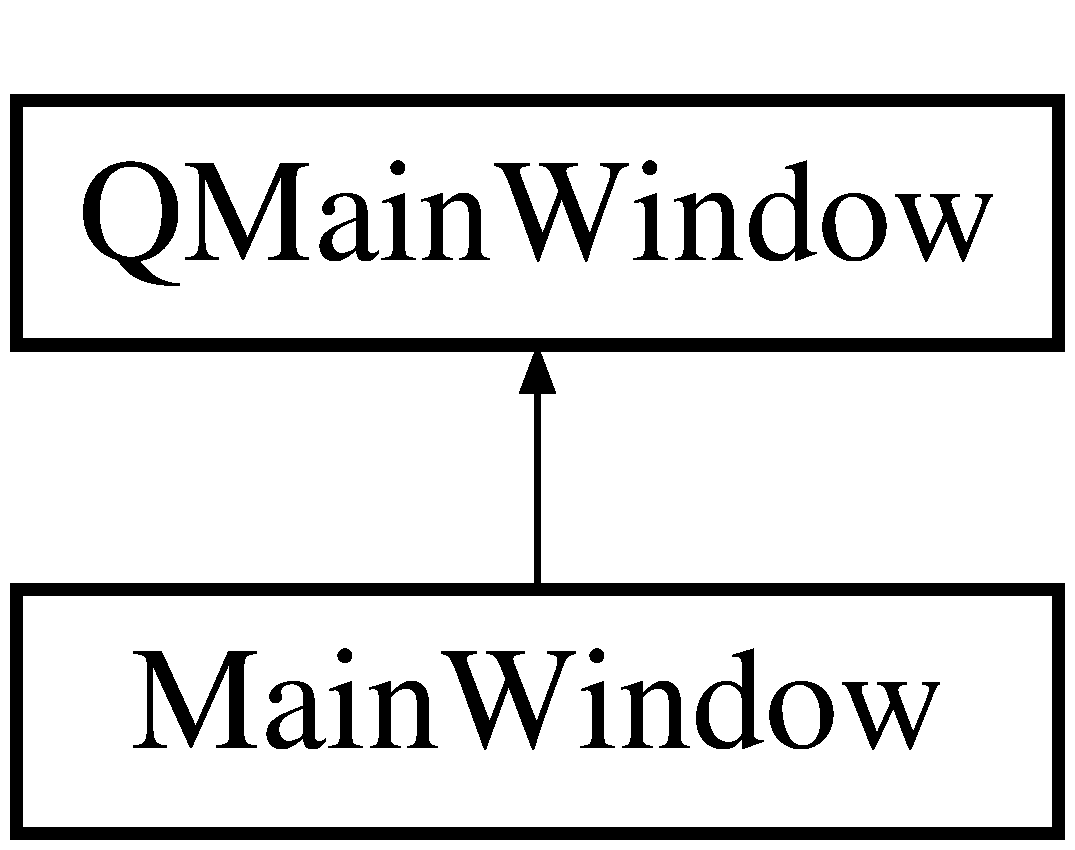
\includegraphics[height=2.000000cm]{class_main_window}
\end{center}
\end{figure}
\subsection*{Public Member Functions}
\begin{DoxyCompactItemize}
\item 
\hyperlink{class_main_window_a8b244be8b7b7db1b08de2a2acb9409db}{Main\-Window} (Q\-Widget $\ast$parent=0)
\begin{DoxyCompactList}\small\item\em A \hyperlink{class_main_window}{Main\-Window} Object This class creates the Menu U\-I and sets up background music. \end{DoxyCompactList}\item 
void \hyperlink{class_main_window_ab622d7f3b4082b8221185e216991e602}{play\-Again} ()
\begin{DoxyCompactList}\small\item\em Restarts the menu music. \end{DoxyCompactList}\item 
\hyperlink{class_main_window_ae98d00a93bc118200eeef9f9bba1dba7}{$\sim$\-Main\-Window} ()
\begin{DoxyCompactList}\small\item\em A \hyperlink{class_main_window}{Main\-Window} Destructor Destroys the U\-I and Removes the music player and music list for the menu. \end{DoxyCompactList}\end{DoxyCompactItemize}
\subsection*{Friends}
\begin{DoxyCompactItemize}
\item 
class \hyperlink{class_main_window_a56592566d22f2b39f7d090a5001d3988}{Game\-Screen}
\end{DoxyCompactItemize}


\subsection{Constructor \& Destructor Documentation}
\hypertarget{class_main_window_a8b244be8b7b7db1b08de2a2acb9409db}{\index{Main\-Window@{Main\-Window}!Main\-Window@{Main\-Window}}
\index{Main\-Window@{Main\-Window}!MainWindow@{Main\-Window}}
\subsubsection[{Main\-Window}]{\setlength{\rightskip}{0pt plus 5cm}Main\-Window\-::\-Main\-Window (
\begin{DoxyParamCaption}
\item[{Q\-Widget $\ast$}]{parent = {\ttfamily 0}}
\end{DoxyParamCaption}
)\hspace{0.3cm}{\ttfamily [explicit]}}}\label{class_main_window_a8b244be8b7b7db1b08de2a2acb9409db}


A \hyperlink{class_main_window}{Main\-Window} Object This class creates the Menu U\-I and sets up background music. 

\hypertarget{class_main_window_ae98d00a93bc118200eeef9f9bba1dba7}{\index{Main\-Window@{Main\-Window}!$\sim$\-Main\-Window@{$\sim$\-Main\-Window}}
\index{$\sim$\-Main\-Window@{$\sim$\-Main\-Window}!MainWindow@{Main\-Window}}
\subsubsection[{$\sim$\-Main\-Window}]{\setlength{\rightskip}{0pt plus 5cm}Main\-Window\-::$\sim$\-Main\-Window (
\begin{DoxyParamCaption}
{}
\end{DoxyParamCaption}
)}}\label{class_main_window_ae98d00a93bc118200eeef9f9bba1dba7}


A \hyperlink{class_main_window}{Main\-Window} Destructor Destroys the U\-I and Removes the music player and music list for the menu. 



\subsection{Member Function Documentation}
\hypertarget{class_main_window_ab622d7f3b4082b8221185e216991e602}{\index{Main\-Window@{Main\-Window}!play\-Again@{play\-Again}}
\index{play\-Again@{play\-Again}!MainWindow@{Main\-Window}}
\subsubsection[{play\-Again}]{\setlength{\rightskip}{0pt plus 5cm}void Main\-Window\-::play\-Again (
\begin{DoxyParamCaption}
{}
\end{DoxyParamCaption}
)}}\label{class_main_window_ab622d7f3b4082b8221185e216991e602}


Restarts the menu music. 

\begin{DoxyRefDesc}{Bug}
\item[\hyperlink{bug__bug000002}{Bug}]this is currently not being called Starts up the main menu music. This is to be used after Game music is stopped. \end{DoxyRefDesc}


\subsection{Friends And Related Function Documentation}
\hypertarget{class_main_window_a56592566d22f2b39f7d090a5001d3988}{\index{Main\-Window@{Main\-Window}!Game\-Screen@{Game\-Screen}}
\index{Game\-Screen@{Game\-Screen}!MainWindow@{Main\-Window}}
\subsubsection[{Game\-Screen}]{\setlength{\rightskip}{0pt plus 5cm}friend class {\bf Game\-Screen}\hspace{0.3cm}{\ttfamily [friend]}}}\label{class_main_window_a56592566d22f2b39f7d090a5001d3988}


The documentation for this class was generated from the following files\-:\begin{DoxyCompactItemize}
\item 
\hyperlink{mainwindow_8h}{mainwindow.\-h}\item 
\hyperlink{mainwindow_8cpp}{mainwindow.\-cpp}\end{DoxyCompactItemize}

\hypertarget{class_wall}{\section{Wall Class Reference}
\label{class_wall}\index{Wall@{Wall}}
}


The \hyperlink{class_wall}{Wall} class of Bombster used to create and destroy non-\/destructable walls in the game.  




{\ttfamily \#include $<$wall.\-h$>$}

Inheritance diagram for Wall\-:\begin{figure}[H]
\begin{center}
\leavevmode
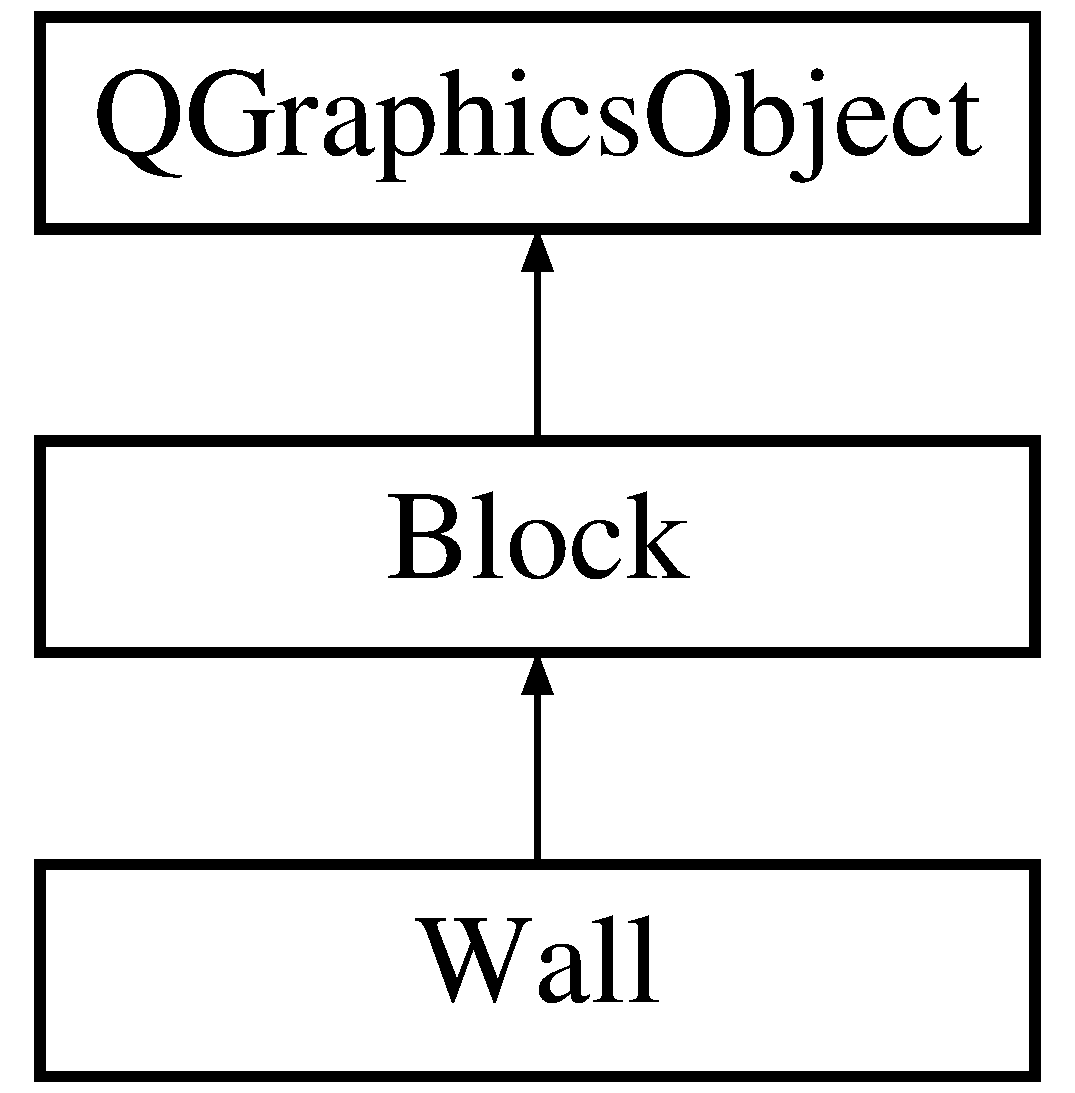
\includegraphics[height=3.000000cm]{class_wall}
\end{center}
\end{figure}
\subsection*{Public Member Functions}
\begin{DoxyCompactItemize}
\item 
\hyperlink{class_wall_a23004a32bc2720e18793d6db6a5f0fd5}{Wall} (int x=0, int y=0)
\item 
\hyperlink{class_wall_a9a2992f2b533e1c160513d1e719f920c}{$\sim$\-Wall} ()
\item 
void \hyperlink{class_wall_aae57ed47f7d5d58b513d2ebd8feb8057}{paint} (Q\-Painter $\ast$painter, const Q\-Style\-Option\-Graphics\-Item $\ast$option, Q\-Widget $\ast$widget)
\item 
Q\-Rect\-F \hyperlink{class_wall_aae7888200bcd5afb12b24110886366a0}{bounding\-Rect} () const 
\item 
int \hyperlink{class_wall_ab31daa81d4977819c8e231621c7573d7}{type} () const 
\end{DoxyCompactItemize}
\subsection*{Additional Inherited Members}


\subsection{Detailed Description}
The \hyperlink{class_wall}{Wall} class of Bombster used to create and destroy non-\/destructable walls in the game. 

Inherits \hyperlink{class_block}{Block} 

\subsection{Constructor \& Destructor Documentation}
\hypertarget{class_wall_a23004a32bc2720e18793d6db6a5f0fd5}{\index{Wall@{Wall}!Wall@{Wall}}
\index{Wall@{Wall}!Wall@{Wall}}
\subsubsection[{Wall}]{\setlength{\rightskip}{0pt plus 5cm}Wall\-::\-Wall (
\begin{DoxyParamCaption}
\item[{int}]{x = {\ttfamily 0}, }
\item[{int}]{y = {\ttfamily 0}}
\end{DoxyParamCaption}
)}}\label{class_wall_a23004a32bc2720e18793d6db6a5f0fd5}
\hypertarget{class_wall_a9a2992f2b533e1c160513d1e719f920c}{\index{Wall@{Wall}!$\sim$\-Wall@{$\sim$\-Wall}}
\index{$\sim$\-Wall@{$\sim$\-Wall}!Wall@{Wall}}
\subsubsection[{$\sim$\-Wall}]{\setlength{\rightskip}{0pt plus 5cm}Wall\-::$\sim$\-Wall (
\begin{DoxyParamCaption}
{}
\end{DoxyParamCaption}
)}}\label{class_wall_a9a2992f2b533e1c160513d1e719f920c}


\subsection{Member Function Documentation}
\hypertarget{class_wall_aae7888200bcd5afb12b24110886366a0}{\index{Wall@{Wall}!bounding\-Rect@{bounding\-Rect}}
\index{bounding\-Rect@{bounding\-Rect}!Wall@{Wall}}
\subsubsection[{bounding\-Rect}]{\setlength{\rightskip}{0pt plus 5cm}Q\-Rect\-F Wall\-::bounding\-Rect (
\begin{DoxyParamCaption}
{}
\end{DoxyParamCaption}
) const\hspace{0.3cm}{\ttfamily [virtual]}}}\label{class_wall_aae7888200bcd5afb12b24110886366a0}


Reimplemented from \hyperlink{class_block_aee4444b92a82f5a8080e9019ef1e554d}{Block}.

\hypertarget{class_wall_aae57ed47f7d5d58b513d2ebd8feb8057}{\index{Wall@{Wall}!paint@{paint}}
\index{paint@{paint}!Wall@{Wall}}
\subsubsection[{paint}]{\setlength{\rightskip}{0pt plus 5cm}void Wall\-::paint (
\begin{DoxyParamCaption}
\item[{Q\-Painter $\ast$}]{painter, }
\item[{const Q\-Style\-Option\-Graphics\-Item $\ast$}]{option, }
\item[{Q\-Widget $\ast$}]{widget}
\end{DoxyParamCaption}
)\hspace{0.3cm}{\ttfamily [virtual]}}}\label{class_wall_aae57ed47f7d5d58b513d2ebd8feb8057}


Reimplemented from \hyperlink{class_block_a8f526f6d76bf11afae85d8b23239cce2}{Block}.

\hypertarget{class_wall_ab31daa81d4977819c8e231621c7573d7}{\index{Wall@{Wall}!type@{type}}
\index{type@{type}!Wall@{Wall}}
\subsubsection[{type}]{\setlength{\rightskip}{0pt plus 5cm}int Wall\-::type (
\begin{DoxyParamCaption}
{}
\end{DoxyParamCaption}
) const\hspace{0.3cm}{\ttfamily [virtual]}}}\label{class_wall_ab31daa81d4977819c8e231621c7573d7}


Reimplemented from \hyperlink{class_block_a915a8196ec94388fb2aae7788af88705}{Block}.



The documentation for this class was generated from the following files\-:\begin{DoxyCompactItemize}
\item 
\hyperlink{wall_8h}{wall.\-h}\item 
\hyperlink{wall_8cpp}{wall.\-cpp}\end{DoxyCompactItemize}

\hypertarget{class_world}{\section{World Class Reference}
\label{class_world}\index{World@{World}}
}
\subsection*{Public Member Functions}
\begin{DoxyCompactItemize}
\item 
\hypertarget{class_world_a83f49e35b8f8b33f14198e87b2fa7312}{void {\bfseries key\-Handler} (int k)}\label{class_world_a83f49e35b8f8b33f14198e87b2fa7312}

\item 
\hypertarget{class_world_a08d405bfe0cef56b06f731addeb22bcf}{void {\bfseries draw\-World} (Q\-Painter $\ast$painter)}\label{class_world_a08d405bfe0cef56b06f731addeb22bcf}

\item 
\hypertarget{class_world_ab44648ec788ea8dfe063a1fce7f86026}{int {\bfseries get\-Blocksize} ()}\label{class_world_ab44648ec788ea8dfe063a1fce7f86026}

\item 
\hypertarget{class_world_a43fe0009fa77b79202cd3ef7e8e7af5f}{int {\bfseries get\-Worldsize} ()}\label{class_world_a43fe0009fa77b79202cd3ef7e8e7af5f}

\item 
\hypertarget{class_world_a66856566fadcf64eba71f5e3ccc790df}{\hyperlink{class_character}{Character} $\ast$ {\bfseries get\-Player} ()}\label{class_world_a66856566fadcf64eba71f5e3ccc790df}

\item 
\hypertarget{class_world_a24f0eab80a2a3b6bc983f58fa2adaa55}{\hyperlink{class_block}{Block} $\ast$ {\bfseries get\-Test\-Block} (int x, int y)}\label{class_world_a24f0eab80a2a3b6bc983f58fa2adaa55}

\end{DoxyCompactItemize}


The documentation for this class was generated from the following files\-:\begin{DoxyCompactItemize}
\item 
world.\-h\item 
world.\-cpp\end{DoxyCompactItemize}

\chapter{File Documentation}
\hypertarget{block_8cpp}{\section{block.\-cpp File Reference}
\label{block_8cpp}\index{block.\-cpp@{block.\-cpp}}
}
{\ttfamily \#include \char`\"{}Block.\-h\char`\"{}}\\*
{\ttfamily \#include $<$iostream$>$}\\*

\hypertarget{block_8h}{\section{block.\-h File Reference}
\label{block_8h}\index{block.\-h@{block.\-h}}
}
{\ttfamily \#include $<$Q\-Painter$>$}\\*
{\ttfamily \#include $<$Q\-Graphics\-Object$>$}\\*
{\ttfamily \#include $<$Q\-Image$>$}\\*
\subsection*{Classes}
\begin{DoxyCompactItemize}
\item 
class \hyperlink{class_block}{Block}
\begin{DoxyCompactList}\small\item\em The \hyperlink{class_block}{Block} class of Bombster used as a base for the game grid. \end{DoxyCompactList}\end{DoxyCompactItemize}

\hypertarget{bomb_8cpp}{\section{bomb.\-cpp File Reference}
\label{bomb_8cpp}\index{bomb.\-cpp@{bomb.\-cpp}}
}
{\ttfamily \#include \char`\"{}bomb.\-h\char`\"{}}\\*
{\ttfamily \#include $<$iostream$>$}\\*
{\ttfamily \#include $<$vector$>$}\\*
{\ttfamily \#include $<$Q\-Timer$>$}\\*

\hypertarget{bomb_8h}{\section{bomb.\-h File Reference}
\label{bomb_8h}\index{bomb.\-h@{bomb.\-h}}
}
{\ttfamily \#include $<$Q\-Painter$>$}\\*
{\ttfamily \#include $<$Q\-Image$>$}\\*
{\ttfamily \#include $<$Q\-Graphics\-Object$>$}\\*
{\ttfamily \#include $<$Q\-Graphics\-Scene$>$}\\*
{\ttfamily \#include $<$Q\-Object$>$}\\*
{\ttfamily \#include $<$Q\-Sound$>$}\\*
{\ttfamily \#include \char`\"{}explosion.\-h\char`\"{}}\\*
\subsection*{Classes}
\begin{DoxyCompactItemize}
\item 
class \hyperlink{class_bomb}{Bomb}
\begin{DoxyCompactList}\small\item\em The \hyperlink{class_bomb}{Bomb} class of Bombster used for destruction of blocks and players in game. \end{DoxyCompactList}\end{DoxyCompactItemize}

\hypertarget{boxes_8cpp}{\section{boxes.\-cpp File Reference}
\label{boxes_8cpp}\index{boxes.\-cpp@{boxes.\-cpp}}
}
{\ttfamily \#include \char`\"{}boxes.\-h\char`\"{}}\\*
{\ttfamily \#include $<$iostream$>$}\\*

\hypertarget{boxes_8h}{\section{boxes.\-h File Reference}
\label{boxes_8h}\index{boxes.\-h@{boxes.\-h}}
}
{\ttfamily \#include \char`\"{}block.\-h\char`\"{}}\\*
\subsection*{Classes}
\begin{DoxyCompactItemize}
\item 
class \hyperlink{classboxes}{boxes}
\begin{DoxyCompactList}\small\item\em The Boxes class of Bombster used. \end{DoxyCompactList}\end{DoxyCompactItemize}

\hypertarget{character_8cpp}{\section{character.\-cpp File Reference}
\label{character_8cpp}\index{character.\-cpp@{character.\-cpp}}
}
{\ttfamily \#include \char`\"{}character.\-h\char`\"{}}\\*
{\ttfamily \#include $<$iostream$>$}\\*
{\ttfamily \#include $<$Q\-Timer$>$}\\*

\hypertarget{character_8h}{\section{character.\-h File Reference}
\label{character_8h}\index{character.\-h@{character.\-h}}
}
{\ttfamily \#include \char`\"{}bomb.\-h\char`\"{}}\\*
{\ttfamily \#include $<$Q\-Painter$>$}\\*
{\ttfamily \#include $<$Q\-Image$>$}\\*
{\ttfamily \#include $<$Q\-Graphics\-Object$>$}\\*
{\ttfamily \#include $<$Q\-Graphics\-Scene$>$}\\*
{\ttfamily \#include \char`\"{}block.\-h\char`\"{}}\\*
{\ttfamily \#include \char`\"{}wall.\-h\char`\"{}}\\*
{\ttfamily \#include $<$Q\-List$>$}\\*
{\ttfamily \#include $<$typeinfo$>$}\\*
{\ttfamily \#include $<$iostream$>$}\\*
{\ttfamily \#include $<$string$>$}\\*
\subsection*{Classes}
\begin{DoxyCompactItemize}
\item 
class \hyperlink{class_character}{Character}
\begin{DoxyCompactList}\small\item\em The \hyperlink{class_character}{Character} class of Bombster used to create a movable player in the world. \end{DoxyCompactList}\end{DoxyCompactItemize}

\hypertarget{dwall_8cpp}{\section{dwall.\-cpp File Reference}
\label{dwall_8cpp}\index{dwall.\-cpp@{dwall.\-cpp}}
}
{\ttfamily \#include \char`\"{}dwall.\-h\char`\"{}}\\*
{\ttfamily \#include $<$iostream$>$}\\*

\hypertarget{dwall_8h}{\section{dwall.\-h File Reference}
\label{dwall_8h}\index{dwall.\-h@{dwall.\-h}}
}
{\ttfamily \#include \char`\"{}block.\-h\char`\"{}}\\*
\subsection*{Classes}
\begin{DoxyCompactItemize}
\item 
class \hyperlink{classd_wall}{d\-Wall}
\begin{DoxyCompactList}\small\item\em The \hyperlink{classd_wall}{d\-Wall} class of Bombster used a destructable wall in the game. \end{DoxyCompactList}\end{DoxyCompactItemize}

\hypertarget{explosion_8cpp}{\section{explosion.\-cpp File Reference}
\label{explosion_8cpp}\index{explosion.\-cpp@{explosion.\-cpp}}
}
{\ttfamily \#include \char`\"{}explosion.\-h\char`\"{}}\\*
{\ttfamily \#include $<$iostream$>$}\\*
{\ttfamily \#include $<$Q\-Painter$>$}\\*

\hypertarget{explosion_8h}{\section{explosion.\-h File Reference}
\label{explosion_8h}\index{explosion.\-h@{explosion.\-h}}
}
{\ttfamily \#include $<$Q\-Graphics\-Item$>$}\\*
\subsection*{Classes}
\begin{DoxyCompactItemize}
\item 
class \hyperlink{classexplosion}{explosion}
\begin{DoxyCompactList}\small\item\em The Explosion class of Bombster used in addition to the bomb class to remove blocks/players. \end{DoxyCompactList}\end{DoxyCompactItemize}

\hypertarget{gamescreen_8cpp}{\section{gamescreen.\-cpp File Reference}
\label{gamescreen_8cpp}\index{gamescreen.\-cpp@{gamescreen.\-cpp}}
}
{\ttfamily \#include \char`\"{}gamescreen.\-h\char`\"{}}\\*
{\ttfamily \#include \char`\"{}mainwindow.\-h\char`\"{}}\\*
{\ttfamily \#include \char`\"{}ui\-\_\-gamescreen.\-h\char`\"{}}\\*
{\ttfamily \#include $<$Q\-Key\-Event$>$}\\*
{\ttfamily \#include $<$Q\-Timer$>$}\\*
{\ttfamily \#include $<$Q\-Graphics\-Scene$>$}\\*

\hypertarget{gamescreen_8h}{\section{gamescreen.\-h File Reference}
\label{gamescreen_8h}\index{gamescreen.\-h@{gamescreen.\-h}}
}
{\ttfamily \#include $<$Q\-Main\-Window$>$}\\*
{\ttfamily \#include \char`\"{}world.\-h\char`\"{}}\\*
{\ttfamily \#include $<$Q\-Media\-Player$>$}\\*
{\ttfamily \#include $<$Q\-Media\-Playlist$>$}\\*
{\ttfamily \#include $<$Q\-Close\-Event$>$}\\*
\subsection*{Classes}
\begin{DoxyCompactItemize}
\item 
class \hyperlink{class_game_screen}{Game\-Screen}
\begin{DoxyCompactList}\small\item\em The Gamescreen class of Bombster used to create a new game. \end{DoxyCompactList}\end{DoxyCompactItemize}
\subsection*{Namespaces}
\begin{DoxyCompactItemize}
\item 
\hyperlink{namespace_ui}{Ui}
\end{DoxyCompactItemize}

\hypertarget{infoscreen_8cpp}{\section{infoscreen.\-cpp File Reference}
\label{infoscreen_8cpp}\index{infoscreen.\-cpp@{infoscreen.\-cpp}}
}
{\ttfamily \#include \char`\"{}infoscreen.\-h\char`\"{}}\\*
{\ttfamily \#include \char`\"{}ui\-\_\-infoscreen.\-h\char`\"{}}\\*

\hypertarget{infoscreen_8h}{\section{infoscreen.\-h File Reference}
\label{infoscreen_8h}\index{infoscreen.\-h@{infoscreen.\-h}}
}
{\ttfamily \#include $<$Q\-Dialog$>$}\\*
\subsection*{Classes}
\begin{DoxyCompactItemize}
\item 
class \hyperlink{class_info_screen}{Info\-Screen}
\end{DoxyCompactItemize}
\subsection*{Namespaces}
\begin{DoxyCompactItemize}
\item 
\hyperlink{namespace_ui}{Ui}
\end{DoxyCompactItemize}

\hypertarget{main_8cpp}{\section{main.\-cpp File Reference}
\label{main_8cpp}\index{main.\-cpp@{main.\-cpp}}
}
{\ttfamily \#include \char`\"{}mainwindow.\-h\char`\"{}}\\*
{\ttfamily \#include $<$Q\-Application$>$}\\*
\subsection*{Functions}
\begin{DoxyCompactItemize}
\item 
int \hyperlink{main_8cpp_a0ddf1224851353fc92bfbff6f499fa97}{main} (int argc, char $\ast$argv\mbox{[}$\,$\mbox{]})
\begin{DoxyCompactList}\small\item\em Creates a Main Menu This begins the program and creates a \hyperlink{class_main_window}{Main\-Window} object. \end{DoxyCompactList}\end{DoxyCompactItemize}


\subsection{Function Documentation}
\hypertarget{main_8cpp_a0ddf1224851353fc92bfbff6f499fa97}{\index{main.\-cpp@{main.\-cpp}!main@{main}}
\index{main@{main}!main.cpp@{main.\-cpp}}
\subsubsection[{main}]{\setlength{\rightskip}{0pt plus 5cm}int main (
\begin{DoxyParamCaption}
\item[{int}]{argc, }
\item[{char $\ast$}]{argv\mbox{[}$\,$\mbox{]}}
\end{DoxyParamCaption}
)}}\label{main_8cpp_a0ddf1224851353fc92bfbff6f499fa97}


Creates a Main Menu This begins the program and creates a \hyperlink{class_main_window}{Main\-Window} object. 


\hypertarget{mainwindow_8cpp}{\section{mainwindow.\-cpp File Reference}
\label{mainwindow_8cpp}\index{mainwindow.\-cpp@{mainwindow.\-cpp}}
}
{\ttfamily \#include \char`\"{}mainwindow.\-h\char`\"{}}\\*
{\ttfamily \#include \char`\"{}ui\-\_\-mainwindow.\-h\char`\"{}}\\*

\hypertarget{mainwindow_8h}{\section{mainwindow.\-h File Reference}
\label{mainwindow_8h}\index{mainwindow.\-h@{mainwindow.\-h}}
}
{\ttfamily \#include $<$Q\-Main\-Window$>$}\\*
{\ttfamily \#include \char`\"{}gamescreen.\-h\char`\"{}}\\*
{\ttfamily \#include \char`\"{}infoscreen.\-h\char`\"{}}\\*
{\ttfamily \#include $<$Q\-Media\-Player$>$}\\*
{\ttfamily \#include $<$Q\-Media\-Playlist$>$}\\*
\subsection*{Classes}
\begin{DoxyCompactItemize}
\item 
class \hyperlink{class_main_window}{Main\-Window}
\begin{DoxyCompactList}\small\item\em The \hyperlink{class_main_window}{Main\-Window} class of Bombster used at the start of program as a menu. \end{DoxyCompactList}\end{DoxyCompactItemize}
\subsection*{Namespaces}
\begin{DoxyCompactItemize}
\item 
\hyperlink{namespace_ui}{Ui}
\end{DoxyCompactItemize}

\hypertarget{wall_8cpp}{\section{wall.\-cpp File Reference}
\label{wall_8cpp}\index{wall.\-cpp@{wall.\-cpp}}
}
{\ttfamily \#include \char`\"{}wall.\-h\char`\"{}}\\*

\hypertarget{wall_8h}{\section{wall.\-h File Reference}
\label{wall_8h}\index{wall.\-h@{wall.\-h}}
}
{\ttfamily \#include \char`\"{}block.\-h\char`\"{}}\\*
{\ttfamily \#include $<$iostream$>$}\\*
\subsection*{Classes}
\begin{DoxyCompactItemize}
\item 
class \hyperlink{class_wall}{Wall}
\end{DoxyCompactItemize}

\hypertarget{world_8cpp}{\section{world.\-cpp File Reference}
\label{world_8cpp}\index{world.\-cpp@{world.\-cpp}}
}
{\ttfamily \#include \char`\"{}world.\-h\char`\"{}}\\*

\hypertarget{world_8h}{\section{world.\-h File Reference}
\label{world_8h}\index{world.\-h@{world.\-h}}
}
{\ttfamily \#include $<$Q\-Font$>$}\\*
{\ttfamily \#include $<$Q\-Pen$>$}\\*
{\ttfamily \#include $<$Q\-Brush$>$}\\*
{\ttfamily \#include $<$Q\-Widget$>$}\\*
{\ttfamily \#include $<$Qt\-Gui$>$}\\*
{\ttfamily \#include $<$Q\-Painter$>$}\\*
{\ttfamily \#include \char`\"{}Block.\-h\char`\"{}}\\*
{\ttfamily \#include \char`\"{}bomb.\-h\char`\"{}}\\*
{\ttfamily \#include \char`\"{}character.\-h\char`\"{}}\\*
{\ttfamily \#include $<$Q\-Key\-Event$>$}\\*
{\ttfamily \#include $<$Q\-Image$>$}\\*
{\ttfamily \#include \char`\"{}wall.\-h\char`\"{}}\\*
{\ttfamily \#include \char`\"{}dwall.\-h\char`\"{}}\\*
{\ttfamily \#include $<$iostream$>$}\\*
{\ttfamily \#include $<$stdlib.\-h$>$}\\*
\subsection*{Classes}
\begin{DoxyCompactItemize}
\item 
class \hyperlink{class_world}{World}
\begin{DoxyCompactList}\small\item\em The \hyperlink{class_world}{World} class of Bombster used to create a new game world. \end{DoxyCompactList}\end{DoxyCompactItemize}

%--- End generated contents ---

% Index
\newpage
\phantomsection
\addcontentsline{toc}{part}{Index}
\printindex

\end{document}
